% =====================================================================
%  PAPER I -- What Authenticity Costs in Metres:
%  A Certified Budget for Cryptography and Sensing in UAV Navigation
%
%  Target venue : IEEE Symposium on Security and Privacy (main track)
%  Class        : IEEEtran (conference). Overleaf ships IEEEtran.
%  Build        : latexmk -pdf main.tex      (pdfLaTeX + BibTeX)
%
%  Every number quoted in the text is a macro from numbers.tex, generated
%  by paperI/experiments/make_numbers.py from the committed result CSVs.
%  Every plotted point is read from figdata/*.dat. Do not edit numbers by
%  hand: re-run paperI/experiments/run_all.sh instead.
% =====================================================================
\documentclass[conference,letterpaper,10pt]{IEEEtran}
\IEEEoverridecommandlockouts
\usepackage{mathptmx}
\usepackage{cite}
\usepackage{amsmath,amssymb,amsfonts}
\usepackage{amsthm}
\usepackage{graphicx}
\usepackage{booktabs}
\usepackage{tabularx}
\usepackage{array}
\usepackage{multirow}
\usepackage{xcolor}
\usepackage{tikz}
\usepackage{pgfplots}
\pgfplotsset{compat=1.17}
\usetikzlibrary{arrows.meta,positioning,fit,backgrounds,shapes.geometric,calc}
\usepackage{algorithm}
\usepackage{algpseudocode}
\usepackage{enumitem}
\usepackage[hidelinks]{hyperref}

% AUTO-GENERATED by paperI/experiments/make_numbers.py -- do not edit
\newcommand{\nAmBusMLk}{18.1}
\newcommand{\nAmBusMLone}{65.3}
\newcommand{\nAmDauthMLk}{820}
\newcommand{\nAmaxEd}{0.885}
\newcommand{\nAmaxFDEd}{0.897}
\newcommand{\nAmaxFDFal}{0.880}
\newcommand{\nAmaxFDML}{0.826}
\newcommand{\nAmaxFDMac}{0.899}
\newcommand{\nAmaxFDSLHs}{0.660}
\newcommand{\nAmaxFal}{0.747}
\newcommand{\nAmaxML}{0.347}
\newcommand{\nAmaxMac}{0.896}
\newcommand{\nAmaxSLHs}{n/a}
\newcommand{\nAsatEd}{0.105}
\newcommand{\nAsatFDEd}{0.025}
\newcommand{\nAsatFDFal}{0.491}
\newcommand{\nAsatFDML}{0.811}
\newcommand{\nAsatFDMac}{0.674}
\newcommand{\nAsatFDSLHs}{0.069}
\newcommand{\nAsatFal}{3.561}
\newcommand{\nAsatML}{5.981}
\newcommand{\nAsatMac}{1.681}
\newcommand{\nAsatSLHs}{0.512}
\newcommand{\nCbnCons}{114}
\newcommand{\nCbnHead}{264}
\newcommand{\nCbnSec}{581}
\newcommand{\nCopCons}{160}
\newcommand{\nCopHead}{371}
\newcommand{\nCopSec}{816}
\newcommand{\nDESmaxEd}{2.61}
\newcommand{\nDESmaxML}{62.72}
\newcommand{\nDESn}{253{,}741}
\newcommand{\nDESok}{all}
\newcommand{\nDRb}{-0.014}
\newcommand{\nDRn}{45}
\newcommand{\nDRrmse}{0.16}
\newcommand{\nDRvzero}{0.857}
\newcommand{\nDauthCertEd}{9.1}
\newcommand{\nDauthCertFDEd}{8.7}
\newcommand{\nDauthCertFDFal}{54.4}
\newcommand{\nDauthCertFDML}{68.1}
\newcommand{\nDauthCertFDMac}{4.9}
\newcommand{\nDauthCertFDTeslaA}{64.9}
\newcommand{\nDauthCertFDTeslaB}{114.9}
\newcommand{\nDauthCertFDTeslaC}{514.9}
\newcommand{\nDauthCertFal}{66.8}
\newcommand{\nDauthCertML}{119.0}
\newcommand{\nDauthCertMac}{4.4}
\newcommand{\nDauthCertTeslaA}{64.6}
\newcommand{\nDauthCertTeslaB}{114.6}
\newcommand{\nDauthCertTeslaC}{514.6}
\newcommand{\nDauthEd}{9.1}
\newcommand{\nDauthFal}{66.8}
\newcommand{\nDauthML}{69.2}
\newcommand{\nDauthMac}{4.4}
\newcommand{\nDauthTeslaA}{64.6}
\newcommand{\nDauthTeslaB}{114.6}
\newcommand{\nDauthTeslaC}{514.6}
\newcommand{\nEmult}{3.259}
\newcommand{\nFramesEd}{10}
\newcommand{\nFramesFDEd}{2}
\newcommand{\nFramesFDFal}{11}
\newcommand{\nFramesFDML}{39}
\newcommand{\nFramesFDMac}{1}
\newcommand{\nFramesFDSLHf}{272}
\newcommand{\nFramesFDSLHs}{125}
\newcommand{\nFramesFal}{96}
\newcommand{\nFramesML}{346}
\newcommand{\nFramesMac}{3}
\newcommand{\nFramesSLHf}{2442}
\newcommand{\nFramesSLHs}{1123}
\newcommand{\nGammaA}{0.933}
\newcommand{\nGammaRatio}{1.74}
\newcommand{\nGammaRatioP}{1.95}
\newcommand{\nGammaRatioPhi}{2.67}
\newcommand{\nGammaRatioPlo}{1.68}
\newcommand{\nGammaReq}{6.14}
\newcommand{\nGammaU}{1.625}
\newcommand{\nHzCrossEd}{0.260}
\newcommand{\nHzCrossFal}{0.274}
\newcommand{\nHzCrossML}{0.284}
\newcommand{\nHzCrossMac}{0.259}
\newcommand{\nHzCrossTeslaB}{0.283}
\newcommand{\nHzCrossTeslaC}{0.999}
\newcommand{\nHzCrossTeslaD}{1.357}
\newcommand{\nHzDaHalfML}{0.65}
\newcommand{\nHzDiffOpCm}{1}
\newcommand{\nHzDu}{0.46}
\newcommand{\nHzDuHalf}{0.93}
\newcommand{\nHzGainHalfEd}{1.10}
\newcommand{\nHzGainHalfFal}{1.00}
\newcommand{\nHzGainHalfML}{0.91}
\newcommand{\nHzGainHalfMac}{1.11}
\newcommand{\nHzGainHalfTeslaB}{0.92}
\newcommand{\nHzGainHalfTeslaC}{-0.48}
\newcommand{\nHzGainHalfTeslaD}{-2.46}
\newcommand{\nHzGainOpEd}{-3.8}
\newcommand{\nHzGainOpFal}{-9.1}
\newcommand{\nHzGainOpML}{-13.7}
\newcommand{\nHzGainOpMac}{-3.4}
\newcommand{\nHzGainOpTeslaB}{-13.3}
\newcommand{\nHzGainOpTeslaC}{-44.1}
\newcommand{\nHzGainOpTeslaD}{-200.9}
\newcommand{\nHzLossOpEd}{3.8}
\newcommand{\nHzLossOpFal}{9.1}
\newcommand{\nHzLossOpML}{13.7}
\newcommand{\nHzLossOpMac}{3.4}
\newcommand{\nHzLossOpTeslaB}{13.3}
\newcommand{\nHzLossOpTeslaC}{44.1}
\newcommand{\nHzLossOpTeslaD}{200.9}
\newcommand{\nMDcross}{0.91}
\newcommand{\nMLtail}{12.2}
\newcommand{\nMminU}{2.65}
\newcommand{\nPushHundred}{600}
\newcommand{\nPushOne}{16.7}
\newcommand{\nPushTen}{6000}
\newcommand{\nRTAEd}{5.44}
\newcommand{\nRTAML}{63.04}
\newcommand{\nRatioCons}{1.32}
\newcommand{\nRatioHead}{1.74}
\newcommand{\nRatioSec}{2.63}
\newcommand{\nRhoAEd}{1.55}
\newcommand{\nRhoAML}{1.88}
\newcommand{\nRhoAMLCons}{2.48}
\newcommand{\nRhoAMac}{1.53}
\newcommand{\nRhoU}{2.65}
\newcommand{\nRhoivEd}{1.647}
\newcommand{\nRhoivFDEd}{6.842}
\newcommand{\nRhoivFDFal}{0.390}
\newcommand{\nRhoivFDML}{0.226}
\newcommand{\nRhoivFDMac}{0.296}
\newcommand{\nRhoivFDSLHs}{0.647}
\newcommand{\nRhoivFal}{0.054}
\newcommand{\nRhoivML}{0.031}
\newcommand{\nRhoivMac}{0.119}
\newcommand{\nRhoivSLHs}{0.087}
\newcommand{\nRstarEd}{563.1}
\newcommand{\nRstarFDEd}{2339.0}
\newcommand{\nRstarFDFal}{425.3}
\newcommand{\nRstarFDML}{120.0}
\newcommand{\nRstarFDMac}{4678.0}
\newcommand{\nRstarFDSLHf}{17.2}
\newcommand{\nRstarFDSLHs}{37.4}
\newcommand{\nRstarFal}{58.7}
\newcommand{\nRstarML}{16.3}
\newcommand{\nRstarMac}{1877.0}
\newcommand{\nRstarSLHf}{2.3}
\newcommand{\nRstarSLHs}{5.0}
\newcommand{\nRstarTesla}{1407.8}
\newcommand{\nRstarZeroEd}{625.0}
\newcommand{\nRstarZeroFal}{65.1}
\newcommand{\nRstarZeroML}{18.1}
\newcommand{\nRstarZeroMac}{2083.3}
\newcommand{\nRstarZeroSLHf}{2.6}
\newcommand{\nRstarZeroSLHs}{5.6}
\newcommand{\nRtxEd}{5.4}
\newcommand{\nRtxFal}{19.2}
\newcommand{\nRtxML}{63.0}
\newcommand{\nRtxMac}{4.3}
\newcommand{\nRtxTeslaA}{4.5}
\newcommand{\nRtxTeslaB}{4.5}
\newcommand{\nRtxTeslaC}{4.5}
\newcommand{\nSelCells}{512}
\newcommand{\nSelConsDenial}{128}
\newcommand{\nSelConsDenialInf}{32}
\newcommand{\nSelHeadDelay}{128}
\newcommand{\nSelHeadDelayInf}{24}
\newcommand{\nSelHeadDelayNone}{80}
\newcommand{\nSelHeadDenial}{128}
\newcommand{\nSelHeadDenialInf}{24}
\newcommand{\nSelInfeasible}{112}
\newcommand{\nSelRescue}{24}
\newcommand{\nThetaCrossConsEd}{0.014}
\newcommand{\nThetaCrossConsML}{0.186}
\newcommand{\nThetaCrossConsMac}{0.007}
\newcommand{\nThetaCrossHeadEd}{0.006}
\newcommand{\nThetaCrossHeadML}{0.080}
\newcommand{\nThetaCrossHeadMac}{0.003}
\newcommand{\nTsignEd}{1.03}
\newcommand{\nTsignFal}{46.81}
\newcommand{\nTsignML}{4.43}
\newcommand{\nTsignMac}{0.06}
\newcommand{\nTsignSLHf}{767.87}
\newcommand{\nTsignSLHs}{15953.25}
\newcommand{\nTverEd}{2.636}
\newcommand{\nTverFal}{0.827}
\newcommand{\nTverML}{1.694}
\newcommand{\nTverMac}{0.057}
\newcommand{\nTverSLHf}{45.674}
\newcommand{\nTverSLHs}{15.566}
\newcommand{\nTxEd}{1.60}
\newcommand{\nTxFal}{15.36}
\newcommand{\nTxML}{55.36}
\newcommand{\nTxMac}{0.48}
\newcommand{\nTxSLHf}{390.72}
\newcommand{\nTxSLHs}{179.68}
\newcommand{\nUzeroMax}{0.099}


% ---------------- notation -------------------------------------------
\newcommand{\Dauth}{\Delta_{\mathrm{auth}}}
\newcommand{\Deff}{\Delta_{\mathrm{eff}}}
\newcommand{\geff}{\gamma_{\mathrm{eff}}}
\newcommand{\gu}{\gamma_{\mathrm{u}}}
\newcommand{\ga}{\gamma_{\mathrm{a}}}
\newcommand{\du}{\delta_{\mathrm{u}}}
\newcommand{\da}{\delta_{\mathrm{a}}}
\newcommand{\tfresh}{\tau_{\mathrm{fresh}}}
\newcommand{\eclk}{\varepsilon_{\mathrm{clk}}}
\newcommand{\riv}{\rho_{\mathrm{iv}}}
\newcommand{\Rtx}{R_{\mathrm{tx}}}
\newcommand{\tsign}{t_{\mathrm{sign}}}
\newcommand{\tver}{t_{\mathrm{ver}}}
\newcommand{\tproto}{t_{\mathrm{proto}}}
\newcommand{\rstar}{r^{\star}}
\newcommand{\Cf}{C_{\mathrm{f}}}
\newcommand{\thx}{\theta_{\times}}
\newcommand{\prov}[1]{\textsc{\footnotesize #1}}

\newtheorem{proposition}{Proposition}
\newtheorem{theorem}{Theorem}
\newtheorem{lemma}{Lemma}
\newtheorem{corollary}{Corollary}
\theoremstyle{definition}
\newtheorem{definition}{Definition}

\begin{document}

\title{What Authenticity Costs in Metres:\\
A Certified Budget for Cryptography and Sensing in UAV Navigation}

\author{\IEEEauthorblockN{Paper \#XXX}
\IEEEauthorblockA{Submitted for double-blind review}}

\maketitle

% =====================================================================
\begin{abstract}
A recent line of work certifies that an unmanned aerial vehicle (UAV) completes its mission
against an adversary who stays just below an intrusion detector's threshold. The certificate
bounds the position error as the product of three factors: the delay the adversary can hide,
the rate $\gamma$ at which delayed navigation input becomes position error, and a dynamics
factor. We observe that authentication moves the first two factors in opposite directions.
Authenticating a navigation source lowers $\gamma$, because a forged fix is rejected rather
than fused. Signing, transmitting and verifying the authenticator raises the delay. The
certificate is therefore a budget in which cryptography and sensing trade, and it decides
the sign of the trade in metres.

We make this budget explicit and measure both sides. On the sensing side, 674 post-onset
samples from real global positioning system (GPS) spoofing and jamming flights show that a
spoofed estimator degrades up to $\nRatioHead\times$ faster than one fed degraded but honest
fixes. Within the first half-second of staleness, however, the two cannot be told apart. On
the cryptographic side, a response-time analysis of a controller area network (CAN) bus,
using a base load derived from a real UAVCAN capture, shows that the binding cost of
post-quantum signatures (ML-DSA and SLH-DSA, standardised by the US National Institute of
Standards and Technology, NIST) is bus occupancy, not latency. ML-DSA-44 costs $\nDauthCertML$\,ms
per message, yet classic CAN admits only $\nRstarML$ signed messages per second.
SLH-DSA cannot be carried at a usable rate at all.

Four results follow. (i)~Under the certificate's supremum discipline, every per-message
signature scheme that fits on the bus pays across the certified window. Authentication also
rescues the tightest corridor, which the unauthenticated certificate cannot cover.
(ii)~Matched to the horizon the detector actually admits, the data cannot show any benefit
at the parent's operating point. The two error envelopes differ by $\nHzDiffOpCm$\,cm,
well inside measurement noise, and authentication pays only from
$\thx\approx\nHzCrossMac$--$\nHzCrossML$\,s. A sound certificate is therefore not
necessarily a good design oracle. (iii)~Deployed freshness windows of 30--165\,s never bind
against detector-scale delays. Where the signing clock is advanced from GNSS time, as
MAVLink~2 prescribes at GPS lock, a spoofer who pushes that clock forward converts the delay
adversary into a denial adversary. (iv)~An attacker who floods invalid Ed25519 signatures
saturates the verifier using $\nAsatEd$ of the bus. Large post-quantum signatures are
immune on classic CAN, but not on CAN with flexible data rate (CAN FD). A selection rule
returns the cheapest certified configuration. Every number in the paper regenerates from
released data, and a defined set of simulator and hardware experiments replaces each
remaining modelled input.
\end{abstract}

\begin{IEEEkeywords}
UAV security, certified robustness, post-quantum cryptography, broadcast authentication,
CAN bus, GNSS spoofing, real-time analysis
\end{IEEEkeywords}

% =====================================================================
\section{Introduction}
\label{sec:intro}
% =====================================================================
An autonomous unmanned aerial vehicle (UAV) navigates on inputs it does not produce itself.
Satellite fixes from a global navigation satellite system (GNSS) receiver, position reports
relayed by peers in a swarm, and commands from a ground station all arrive over links an
adversary can reach. Two families of defence address this exposure, and they rarely meet.
Cryptographic authentication proves where a message came from. Navigation-message
authentication for GNSS~\cite{gotzelmann2023osnma,anderson2017chimera}, message signing on
the Micro Air Vehicle Link (MAVLink) protocol~\cite{mavlink_signing,koubaa2019mavlink}, and
authentication schemes for the controller area network (CAN)
bus~\cite{nurnberger2016vatican,radu2016leia,pese2021s2can} all belong here. Certified
robustness proves that a navigation stack tolerates a bounded perturbation of its inputs. A
recent composition~\cite{parentpaper} joined an intrusion detector to such a certificate.
For an adversary who delays relayed messages by just less than the detector's threshold
$\theta$, it bounds the worst-case deviation from the planned route as
\begin{equation}
\label{eq:rho-parent}
\rho(\theta)\;=\;\Delta(\theta)\cdot\gamma\cdot e^{LT_c}\;\le\;m ,
\end{equation}
where $\Delta(\theta)$ is the delay the adversary can hide, $\gamma$ the rate (in metres per
second) at which stale input becomes position error, $L$ a Lipschitz constant of the
navigation dynamics, $T_c$ a re-anchoring horizon, and $m$ the lateral margin of the safe
corridor.

\paragraph*{The observation}
Two of the four factors in Eq.~\eqref{eq:rho-parent} are fixed by physics ($L$) and by
regulation ($m$). The other two are security-engineering choices, and authentication moves
them in opposite directions. Authenticating a navigation source lowers $\gamma$, because an
estimator that rejects a forged fix stops absorbing the forger's offset. Authenticating a
message raises $\Delta$, because signing, transmitting and verifying the authenticator take
time, and stale input is stale regardless of why it is stale. Authentication is therefore
both a credit and a debit against one certified budget. Neither the cryptographic nor the
certified-robustness literature can say which effect wins, because the two sides are
measured on different instruments: a cycle counter on a microcontroller and a flight log of
a spoofed receiver.

\paragraph*{This paper}
We write the budget down, derive when authentication increases the certified margin, and
measure both sides on real data and real specifications. The results do not all point the
same way, and the disagreement is itself a finding.
\begin{itemize}[leftmargin=*,itemsep=1pt,topsep=2pt]
\item \textbf{The crossover and its two readings} (Section~\ref{sec:theory},
  Proposition~\ref{pr:crossover}, Theorem~\ref{th:horizon}). Under the parent certificate's
  discipline of one supremum rate per configuration, authentication pays whenever its cost
  $\Dauth$ is below $\Delta(\theta)(\gu/\ga-1)$. With the measured rates, every per-message
  signature scheme that fits on the bus meets this across the certified window. It also
  rescues the 2\,m corridor that the unauthenticated certificate cannot cover:
  $\rho=\nRhoAML$\,m with ML-DSA-44, against $\nRhoU$\,m without. When the rates are matched
  to the horizon the detector actually admits, the picture changes at tight settings. Within
  half a second of staleness, the spoofed and the honest-but-degraded estimators have
  accrued the same error to within $\nHzDiffOpCm$\,cm, so the data cannot show a benefit. On
  the measured envelopes, authentication pays from $\thx=\nHzCrossMac$\,s (a group message authentication code, MAC) to
  $\nHzCrossML$\,s (ML-DSA-44).
\item \textbf{The cost is a cliff, not a slope} (Proposition~\ref{pr:cliff}). We consider
  the post-quantum cryptography (PQC) signatures that NIST standardised as Federal
  Information Processing Standards (FIPS):
  the module-lattice-based digital signature algorithm ML-DSA (FIPS~204)~\cite{fips204} and
  the stateless hash-based SLH-DSA (FIPS~205)~\cite{fips205}. We use a base load derived from
  a real capture of UAVCAN (now DroneCAN, the CAN protocol linking a flight controller to its
  peripherals). On that bus, the worst-case transmission latency of a signed message is flat
  up to an admissible rate $\rstar$ and unbounded beyond it. On classic CAN, $\rstar$ is
  $\nRstarML$/s for ML-DSA-44 and $\nRstarSLHs$/s for SLH-DSA-128s. A discrete-event
  simulation of $\nDESn$ transfers stays within the analytical bound.
\item \textbf{Freshness does not bound delay, and the clock can turn delay into denial}
  (Proposition~\ref{pr:push}). Deployed freshness windows exceed the largest delay the
  detector admits ($Hs=10$\,s) by a factor of 3--17: 60\,s for MAVLink~2, and 30--165\,s for
  Galileo's Open Service Navigation Message Authentication (OSNMA). Where the signing clock
  is advanced from GNSS time, a spoofer who pushes it past the window makes every legitimate
  signed packet stale.
\item \textbf{Induced verification} (Proposition~\ref{pr:iv}). Forged signatures convert
  the defender's verification cost into delay. The classical Edwards-curve signature
  Ed25519 is the scheme most exposed: $\nAsatEd$ of the bus suffices to saturate a verifier
  that has a 20\,\% share of the central processing unit (CPU). ML-DSA-44
  is immune on classic CAN because its signature is too expensive to transmit, but not on
  CAN FD. A slot-budget mitigation bounds the induced delay to one verification.
\item \textbf{A certified selection rule} (Algorithm~\ref{alg:select}). For each detector
  setting, corridor, transport, adversary class and post-quantum requirement, the rule
  returns the cheapest configuration (scheme, batch size, mitigation) that keeps the
  setting certified, or reports that none exists.
\end{itemize}

\paragraph*{Scope and honesty}
The sensing side rests on the same three real flights of one airframe in hover as the
parent~\cite{whelan2020uav}. The authenticated rate is a \emph{proxy}: it is measured on a
jamming flight whose receiver kept a degraded three-dimensional fix, not on an estimator
that rejected GNSS outright (Section~\ref{sec:method}). The cryptographic compute side rests on published Cortex-M
cycle counts scaled to the flight controller's clock. The transport side rests on standard
frame models and a base load derived from frame rates measured on a real bus. Each number carries a provenance tag,
and Section~\ref{sec:runbook} specifies the simulator and hardware experiments that replace
each modelled input. Because every number in this paper is generated from result files, a
replacement propagates to the text without hand editing.

% =====================================================================
\section{Preliminaries and Problem Statement}
\label{sec:prelim}
% =====================================================================
\subsection{The Parent Certificate}
\label{sec:parent}
We inherit the system model and constants of the parent manuscript~\cite{parentpaper},
summarised here so that the paper is self-contained.

\paragraph*{Navigation loop}
A UAV running the PX4 autopilot~\cite{kong2024px4ekf} fuses GNSS fixes, measurements from
an inertial measurement unit (IMU), and barometric height in an extended Kalman filter
(EKF). It also receives relayed corrections from peers over a multi-hop mesh. When GNSS is
gated out, the EKF dead-reckons on the IMU, and its position error grows.

\paragraph*{Residual delay}
A multi-hop forwarding detector $D_\theta$ flags any hop whose forwarding delay exceeds a
per-hop tolerance $\theta$. An adversary controlling $H$ relays on a route can hide at most
\begin{equation}
\label{eq:delta}
\Delta(\theta)\;\le\;H\,\min(\theta,s)
\end{equation}
seconds of delay, where $s$ is the contact-window slack. A delay beyond $s$ misses its
window and is flagged at any threshold. The parent measures $s=5$\,s (cap 4.84\,s over
15{,}392 hops). It also measures a benign residual ceiling of 0.178\,s, below which $\theta$
cannot go without false alarms, and adopts $H=2$ and the operating point $\theta=0.25$\,s.

\paragraph*{Interface rate}
The rate $\gamma$ is estimated with the baseline-corrected estimator
\begin{equation}
\label{eq:gamma-delta}
\gamma_\delta(\tau)\;=\;\frac{e(t_0+\tau)-e(t_0)}{\tau},
\end{equation}
where $e$ is the horizontal position error of the EKF output, $t_0$ the attack onset, and
$\tau$ the staleness. The parent evaluates its certificate at the supremum over all 674
post-onset samples, $\gamma=1.625$\,m/s.

\paragraph*{Tube}
If the navigation drift is $L$-Lipschitz and the filter re-anchors at least once every
$T_c$, Grönwall's inequality~\cite{gronwall1919} bounds the deviation by
Eq.~\eqref{eq:rho-parent}, with $L=1.1814$, $T_c=1$\,s, and hence
$E\triangleq e^{LT_c}=\nEmult$. The corridor family $m\in\{2,5,10,20\}$\,m brackets the
contingency volumes of the Joint Authorities for Rulemaking of Unmanned Systems (JARUS)
Specific Operations Risk Assessment (SORA)~\cite{jarus_sora25}. At $\theta=0.25$\,s the
unauthenticated tube is $\rho=\nRhoU$\,m. The setting is therefore certified for
$m\ge5$\,m but not for $m=2$\,m. We call the set of $\theta$ for which $\rho(\theta)\le m$
the \emph{certified window}. Its lower edge is the benign floor of 0.178\,s.

\subsection{Threat Model}
\label{sec:threat}
We retain the parent's two adversaries and add three. Table~\ref{tab:adversaries}
summarises what authentication does against each.

\begin{table}[t]
\centering
\caption{Adversaries and what authentication buys against each.}
\label{tab:adversaries}
\footnotesize
\begin{tabularx}{\columnwidth}{@{}p{0.27\columnwidth}X@{}}
\toprule
\textbf{Adversary} & \textbf{Effect of authentication} \\
\midrule
$\mathcal{A}_{\mathrm{spoof}}$: forges GNSS or peer position data &
  Forged data fail verification and are rejected. The estimator stops following the forger, so $\gamma$
  falls from $\gu$ to $\ga$. \\
$\mathcal{A}_{\mathrm{delay}}$: compromised relay forwards valid messages late &
  None, unless the signature covers a timestamp and the receiver enforces a freshness
  window $\tfresh$; then the hidden delay is capped at $\tfresh+\eclk$. \\
$\mathcal{A}_{\mathrm{ins}}$: insider holding a group key &
  Group message authentication codes (MACs) give no protection, since the insider can MAC
  anything. Only asymmetric signatures or delayed key disclosure, as in Timed Efficient
  Stream Loss-tolerant Authentication (TESLA), authenticate the source. \\
$\mathcal{A}_{\mathrm{deny}}$: selectively withholds unauthenticated sources beyond $T_c$ &
  Re-anchoring fails. An authenticated source that is still delivered within $T_c$ is
  \emph{necessary} for any certified floor (Proposition~\ref{pr:regimes}). A jammer that
  also denies the authenticated source is outside this model. \\
$\mathcal{A}_{\mathrm{iv}}$: injects transfers with invalid signatures &
  Each costs $\tver$ before rejection, so the defence's cost becomes delay
  (Proposition~\ref{pr:iv}). \\
$\mathcal{A}_{\mathrm{time}}$: shifts the receiver's GNSS-disciplined clock &
  Erodes or inverts the freshness check (Proposition~\ref{pr:push}). \\
\bottomrule
\end{tabularx}
\end{table}

Three points in Table~\ref{tab:adversaries} are easy to get wrong.

\emph{First, a validly signed message forwarded four seconds late is still validly
signed.} Authentication bounds delay only through a timestamp and a freshness check, and
that check is only as good as the receiver's clock.

\emph{Second, the MAVLink~2 signature is a 48-bit truncation of the Secure Hash Algorithm
SHA-256 over a shared
secret, the packet and a timestamp, not a public-key signature}~\cite{mavlink_signing}.
CAN-layer schemes such as vatiCAN~\cite{nurnberger2016vatican}, LeiA~\cite{radu2016leia}
and the CAN~XL security layer (CANsec)~\cite{cia613} are likewise group-keyed. Against a
compromised relay, which holds the key, they authenticate group membership, not origin.
This has been noted for in-vehicle multicast~\cite{macsec_cansec2025}.

\emph{Third, Galileo's Open Service Navigation Message Authentication
(OSNMA)~\cite{gotzelmann2023osnma} authenticates the navigation data, not the ranging
signal.} Receivers must keep their clock within a loose time-synchronisation bound $T_L$ (30\,s
for the authentication-data-and-key-delay types ADKD0 and ADKD4). A meaconer that replays the
signal with a delay inside $T_L$ therefore passes the check~\cite{wang2025osnmaspoof,anderson2024timesync}. For OSNMA, therefore,
$\ga$ against a meaconer equals $\gu$. Our measured $\ga$ applies to forgery that a
verifier can detect.

\paragraph*{Assumptions}
The adversary knows $\theta$, the scheme and the transport. Legitimate authenticated
navigation messages are released periodically at rate $r$ (10\,Hz unless stated). The
adversary's injected CAN frames do not out-prioritise the legitimate stream: a
higher-priority flood is ordinary bus flooding, which identifier-based intrusion detection
on the UAVCAN capture of the Hacking and Countermeasure Research Lab (HCRL) already
handles~\cite{hcrl_uavcan,parentpaper}.

\subsection{Problem Statement}
\label{sec:problem}
Let $\kappa$ be an authentication configuration: a scheme, a batch size $k$ (one signature
per $k$ messages) and a flooding mitigation. Let $\mathcal{T}$ be the transport. The
\emph{certified budget} is
\begin{equation}
\label{eq:budget}
\rho(\theta,\kappa)\;=\;\Deff(\theta,\kappa)\cdot\geff(\kappa)\cdot e^{LT_c}\;\le\;m,
\end{equation}
\begin{equation}
\label{eq:deff}
\Deff(\theta,\kappa,t)\;=\;\min\!\big(\Delta(\theta),\;\tfresh+\eclk(t)\big)\;+\;\Dauth(\kappa,\mathcal{T}),
\end{equation}
with $\geff=\gu$ for unauthenticated and $\geff=\ga$ for authenticated sources. The design
problem is
\begin{equation}
\label{eq:design}
\begin{aligned}
\min_{\kappa\in\mathcal{K}}\ \ & \mathrm{cost}(\kappa)\\
\text{s.t.}\ \ & \rho(\theta,\kappa)\le m,\quad \kappa\ \text{admissible on}\ \mathcal{T},\\
& \kappa\ \text{secure against}\ \mathcal{A},
\end{aligned}
\end{equation}
where admissibility requires bus and processor utilisation below one, and security
requires source authentication against $\mathcal{A}_{\mathrm{ins}}$, post-quantum security
where mandated~\cite{nistir8547}, and resistance to $\mathcal{A}_{\mathrm{iv}}$. We ask five
research questions (RQs):
\begin{description}[leftmargin=2.4em,style=sameline,itemsep=1pt,topsep=2pt]
\item[RQ1] How much does authentication lower $\gamma$, and over which staleness horizon?
\item[RQ2] What does authentication cost in delay on flight-controller-class hardware, and
  is the binding term latency or occupancy?
\item[RQ3] Where is the crossover in $(\theta,\text{scheme},\text{transport})$?
\item[RQ4] Does a freshness window bound the hidden delay under GNSS-coupled clocks?
\item[RQ5] How much delay can an attacker induce through verification, and how much does
  mitigation recover?
\end{description}
Table~\ref{tab:notation} collects the notation. Fig.~\ref{fig:framework} shows how the
answers are assembled.

\begin{table}[t]
\centering
\caption{Notation.}
\label{tab:notation}
\footnotesize
\begin{tabularx}{\columnwidth}{@{}lX@{}}
\toprule
$\theta,\ H,\ s$ & detector tolerance (s), attacker hops, contact-window slack (5\,s) \\
$\Delta(\theta)$ & hidden delay $\le H\min(\theta,s)$ (s) \\
$\Dauth$ & authentication delay: $\tsign+\Rtx+\tver+\tproto$ (s) \\
$\Deff$ & effective delay entering the tube, Eq.~\eqref{eq:deff} \\
$\gu,\ \ga$ & delay-to-position rate, unauthenticated / authenticated (m/s) \\
$\du(\tau),\ \da(\tau)$ & error accrued within staleness $\tau$ (m) \\
$L,\ T_c,\ E$ & Lipschitz constant, re-anchoring horizon, $E=e^{LT_c}$ \\
$m,\ \rho$ & corridor margin, tube radius (m) \\
$C(\theta),\ B(\theta)$ & benefit threshold, affordability budget (s) \\
$\thx$ & smallest $\theta$ at which authentication pays (s) \\
$\sigma,\ n,\ \Cf$ & tag bytes, frames per tag, worst-case frame time \\
$U_0,\ r,\ \rstar$ & base bus load, signed rate, admissible rate \\
$\tfresh,\ \eclk,\ \nu$ & freshness window, clock error, clock push rate \\
$\riv,\ \beta,\ a$ & verification amplification, CPU share, attacker bus share \\
$k$ & batch size (messages per signature) \\
\bottomrule
\end{tabularx}
\end{table}

% =====================================================================
% Fig. 1 -- Methodological framework of the certified budget.
% Four stages left to right; a validation loop returns along the bottom.
% Requires: tikz with arrows.meta, positioning, fit, backgrounds, calc.
% =====================================================================
\begin{figure*}[t]
\centering
\resizebox{\textwidth}{!}{%
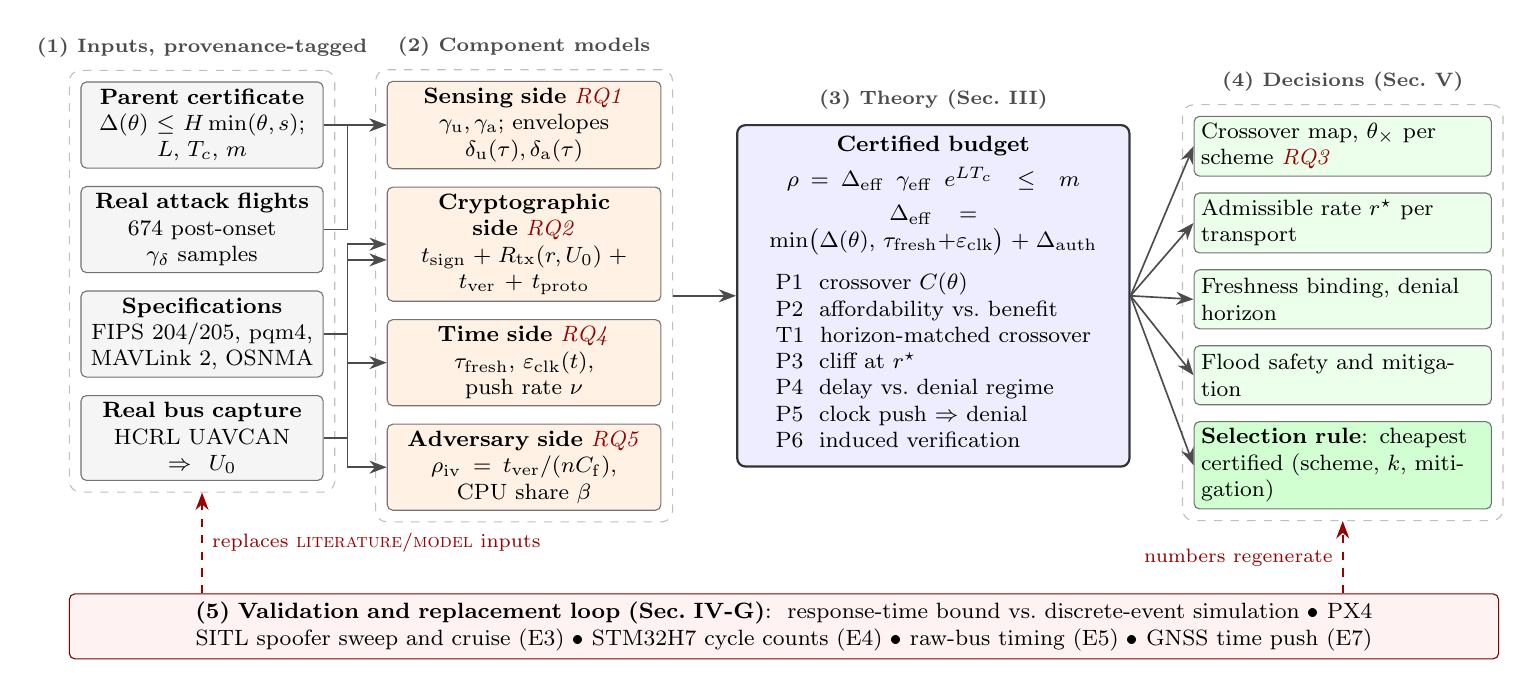
\begin{tikzpicture}[
  font=\footnotesize,
  >={Stealth[length=2.2mm]},
  inbox/.style={draw=black!55, rounded corners=2pt, fill=gray!8, align=center,
                text width=29mm, minimum height=10mm, inner sep=2.5pt},
  model/.style={draw=black!55, rounded corners=2pt, fill=orange!10, align=center,
                text width=33mm, minimum height=10mm, inner sep=2.5pt},
  core/.style={draw=black!80, thick, rounded corners=3pt, fill=blue!7,
               align=center, text width=47mm, inner sep=4pt},
  outbox/.style={draw=black!55, rounded corners=2pt, fill=green!8, align=left,
                 text width=36mm, minimum height=7.5mm, inner sep=2.5pt},
  lane/.style={draw=black!25, dashed, rounded corners=4pt, inner sep=4pt},
  lbl/.style={font=\scriptsize\bfseries, text=black!70},
  rq/.style={font=\scriptsize\bfseries\itshape, text=red!60!black},
  flow/.style={->, draw=black!70, line width=0.6pt},
  fb/.style={->, draw=red!60!black, line width=0.6pt, dashed}
]
% ---------------- (1) inputs ------------------------------------------
\node[inbox] (par) {\textbf{Parent certificate}\\ $\Delta(\theta)\le H\min(\theta,s)$;\ $L,\,T_c,\,m$};
\node[inbox, below=2.2mm of par] (fl) {\textbf{Real attack flights}\\ 674 post-onset $\gamma_\delta$ samples};
\node[inbox, below=2.2mm of fl] (lit) {\textbf{Specifications}\\ FIPS 204/205, pqm4,\\ MAVLink~2, OSNMA};
\node[inbox, below=2.2mm of lit] (bus) {\textbf{Real bus capture}\\ HCRL UAVCAN $\Rightarrow U_0$};
\node[lane, fit=(par)(bus)] (L1) {};
\node[lbl, above=0.4mm of L1] {(1) Inputs, provenance-tagged};

% ---------------- (2) component models --------------------------------
\node[model, right=8mm of par] (sens) {\textbf{Sensing side} \textcolor{red!60!black}{\textit{RQ1}}\\ $\gamma_{\mathrm{u}},\gamma_{\mathrm{a}}$;\ envelopes $\delta_{\mathrm{u}}(\tau),\delta_{\mathrm{a}}(\tau)$};
\node[model, below=2.2mm of sens] (crypto) {\textbf{Cryptographic side} \textcolor{red!60!black}{\textit{RQ2}}\\ $t_{\mathrm{sign}}+R_{\mathrm{tx}}(r,U_0)+t_{\mathrm{ver}}+t_{\mathrm{proto}}$};
\node[model, below=2.2mm of crypto] (clk) {\textbf{Time side} \textcolor{red!60!black}{\textit{RQ4}}\\ $\tau_{\mathrm{fresh}}$,\ $\varepsilon_{\mathrm{clk}}(t)$,\ push rate $\nu$};
\node[model, below=2.2mm of clk] (adv) {\textbf{Adversary side} \textcolor{red!60!black}{\textit{RQ5}}\\ $\rho_{\mathrm{iv}}=t_{\mathrm{ver}}/(nC_{\mathrm{f}})$,\ CPU share $\beta$};
\node[lane, fit=(sens)(adv)] (L2) {};
\node[lbl, above=0.4mm of L2] {(2) Component models};

% ---------------- (3) certified budget --------------------------------
\node[core, right=8mm of L2] (core) {\textbf{Certified budget}\\[3pt]
  $\rho=\Delta_{\mathrm{eff}}\;\gamma_{\mathrm{eff}}\;e^{LT_c}\;\le\;m$\\[3pt]
  $\Delta_{\mathrm{eff}}=\min\!\big(\Delta(\theta),\,\tau_{\mathrm{fresh}}{+}\varepsilon_{\mathrm{clk}}\big)+\Delta_{\mathrm{auth}}$\\[5pt]
  \begin{tabular}{@{}l@{}}
  P1\ \ crossover $C(\theta)$\\
  P2\ \ affordability vs.\ benefit\\
  T1\ \ horizon-matched crossover\\
  P3\ \ cliff at $r^\star$\\
  P4\ \ delay vs.\ denial regime\\
  P5\ \ clock push $\Rightarrow$ denial\\
  P6\ \ induced verification
  \end{tabular}};
\node[lbl, above=0.6mm of core] {(3) Theory (Sec.~III)};

% ---------------- (4) decisions ---------------------------------------
\node[outbox, right=8mm of core, yshift=19mm] (o1) {Crossover map, $\theta_{\times}$ per scheme\ \textcolor{red!60!black}{\textit{RQ3}}};
\node[outbox, below=2mm of o1] (o2) {Admissible rate $r^\star$ per transport};
\node[outbox, below=2mm of o2] (o3) {Freshness binding, denial horizon};
\node[outbox, below=2mm of o3] (o4) {Flood safety and mitigation};
\node[outbox, below=2mm of o4, fill=green!18] (o5) {\textbf{Selection rule}: cheapest certified (scheme, $k$, mitigation)};
\node[lane, fit=(o1)(o5)] (L4) {};
\node[lbl, above=0.4mm of L4] {(4) Decisions (Sec.~V)};

% ---------------- flows -------------------------------------------------
\draw[flow] (fl.east)  -- ++(3mm,0) |- (sens.west);
\draw[flow] (par.east) -- (sens.west |- par.east);
\draw[flow] (lit.east) -- ++(3mm,0) |- (crypto.west);
\draw[flow] (lit.east) -- ++(3mm,0) |- (clk.west);
\draw[flow] (bus.east) -- ++(3mm,0) |- (adv.west);
\draw[flow] (bus.east) -- ++(3mm,0) |- ([yshift=-2mm]crypto.west);
\draw[flow] (L2.east) -- (core.west);
\foreach \o in {o1,o2,o3,o4,o5} \draw[flow] (core.east) -- (\o.west);

% ---------------- (5) validation loop ----------------------------------
\path let \p1=(L1.west), \p2=(L4.east), \p3=(L2.south) in
  node[draw=red!50!black, rounded corners=2pt, fill=red!5, align=center,
       text width={\x2-\x1-8pt}, inner sep=3pt, anchor=north west] (val)
  at (\x1,\y3-9mm)
 {\textbf{(5) Validation and replacement loop (Sec.~IV-G)}:\ \
  response-time bound vs.\ discrete-event simulation\ \textbullet\
  PX4 SITL spoofer sweep and cruise (E3)\ \textbullet\
  STM32H7 cycle counts (E4)\ \textbullet\ raw-bus timing (E5)\ \textbullet\
  GNSS time push (E7)};
\draw[fb] (L1.south |- val.north) -- (L1.south)
  node[midway, right, font=\scriptsize, text=red!60!black]{replaces \textsc{literature}/\textsc{model} inputs};
\draw[fb] (L4.south |- val.north) -- (L4.south)
  node[midway, left, font=\scriptsize, text=red!60!black]{numbers regenerate};
\end{tikzpicture}}
\caption{Methodological framework. (1)~Every input carries a provenance tag: measured on
real flights or buses, derived, taken from a specification, or modelled. (2)~Four component
models quantify the two sides of the trade, sensing and cryptography, together with time
and the flooding adversary. (3)~The certified budget composes them into one inequality in
metres, from which the propositions follow. (4)~The decisions an engineer needs are read off
the budget. (5)~Simulation and hardware experiments replace modelled inputs with measured
ones; because every number in the paper is generated from result files, a replacement
propagates to the text automatically.}
\label{fig:framework}
\end{figure*}


% =====================================================================
\section{Methodology I: The Certified Budget}
\label{sec:theory}
% =====================================================================
The framework (Fig.~\ref{fig:framework}) has five stages: inputs with provenance,
component models, the budget, decisions, and a validation loop. This section develops
stage~(3). Section~\ref{sec:method} develops stages~(2) and~(5). Proofs omitted here are in
Appendix~\ref{app:proofs}.

\subsection{The Crossover under the Supremum Discipline}
Write $E=e^{LT_c}$. In the delay regime, where re-anchoring holds by construction and the
freshness cap does not bind, $\Deff=\Delta(\theta)+\Dauth$.

\begin{proposition}[Crossover]
\label{pr:crossover}
Let authenticating the navigation path change the rate from $\gu$ to $\ga<\gu$ at cost
$\Dauth$. Authentication strictly reduces the certified error if and only if
\begin{equation}
\label{eq:crossover}
\Dauth\;<\;C(\theta)\;\triangleq\;\Delta(\theta)\Big(\frac{\gu}{\ga}-1\Big).
\end{equation}
Equivalently, for $\theta<s$, authentication pays if and only if
$\theta>\thx\triangleq\Dauth/\big(H(\gu/\ga-1)\big)$.
\end{proposition}

\begin{proposition}[More affordable, less beneficial]
\label{pr:afford}
Let $B(\theta)=m/(\ga E)-\Delta(\theta)$ be the largest $\Dauth$ that keeps the
authenticated configuration certified. For $\theta<s$, $B$ decreases with slope $-H$ and
$C$ increases with slope $H(\gu/\ga-1)$. Tightening the detector therefore leaves more room
to afford authentication and less reason to want it.
\end{proposition}

The two halves answer different questions, \emph{can I pay for it?} and \emph{is it worth
paying for?}. An engineer who conflates them will over-invest in cryptography on a platform
whose detector is already tight.

\subsection{The Crossover with a Time-Varying Rate}
Proposition~\ref{pr:crossover} inherits the parent's choice of one supremum rate per
configuration. That choice is sound for certification, but it can mislead design. The
supremum of $\gu$ may be attained at a staleness the detector never admits, and the
unauthenticated configuration is then charged for an error it cannot suffer. We therefore
also state the crossover in terms of the measured error envelope.

\begin{definition}[Error envelope]
For a source in state $x\in\{\mathrm{u},\mathrm{a}\}$, let
$\delta_x(\tau)=\sup_{\tau'\le\tau}\big[e(t_0+\tau')-e(t_0)\big]$, taken over the observed
onsets. By construction, $\delta_x$ is non-decreasing.
\end{definition}

\begin{theorem}[Horizon-matched crossover]
\label{th:horizon}
Under the hypotheses of the parent certificate, with $\gamma\Delta$ replaced by the
envelope $\delta(\Delta)$, authentication strictly reduces the certified tube radius if and
only if
\begin{equation}
\label{eq:horizon}
\da\big(\Delta(\theta)+\Dauth\big)\;<\;\du\big(\Delta(\theta)\big).
\end{equation}
\end{theorem}

\begin{corollary}[Indistinguishability horizon]
\label{co:indist}
If $\du(\tau)\le\da(\tau)$ for all $\tau\le\tau_s$, then authentication cannot pay at any
$\theta$ with $\Delta(\theta)\le\tau_s$, whatever its cost.
\end{corollary}
\begin{proof}
For $\Delta(\theta)\le\tau_s$, monotonicity gives
$\da(\Delta+\Dauth)\ge\da(\Delta)\ge\du(\Delta)$, which contradicts
Eq.~\eqref{eq:horizon}.
\end{proof}

The corollary has a physical reading. A spoofer that walks the fix away gradually, as
spoofers must to stay inside the EKF's innovation gate, needs time to out-run dead
reckoning. Until it does, rejecting its data buys nothing.

\subsection{The Cost Is a Cliff, Not a Slope}
Decompose
\begin{equation}
\label{eq:dauth}
\Dauth=\underbrace{\tsign+\tver}_{\text{compute}}+\underbrace{\Rtx}_{\text{transmission}}+\underbrace{\tproto}_{\text{protocol}},
\end{equation}
where $\Rtx$ is the worst-case response time of the transfer that carries a $\sigma$-byte
authenticator in $n(\sigma)$ frames of worst-case duration $\Cf$.

\begin{proposition}[Cliff]
\label{pr:cliff}
Let signed transfers be released periodically at rate $r$ on a fixed-priority CAN bus with
periodic background traffic of utilisation $U_0$. Then $\Rtx(r)$ is finite for
$r<\rstar$ and infinite for $r\ge\rstar$, where
\begin{equation}
\label{eq:rstar}
\rstar\;=\;\frac{1-U_0}{n(\sigma)\,\Cf}.
\end{equation}
Below $\rstar$, $\Rtx$ is bounded by the busy-period recurrence of Davis
et~al.~\cite{davis2007can}. Ordering schemes by $\sigma$ captures only the transmission
term: schemes that minimise it, such as TESLA, pay instead in $\tproto$ through their
key-disclosure delay.
\end{proposition}

The proposition is a direct consequence of level-$i$ busy-period analysis: the busy period
closes if and only if the total utilisation is below one. Its content for this paper lies
in the magnitudes (Section~\ref{sec:rq2}). Per-message latency is milliseconds, against
budgets of hundreds of milliseconds, so the binding constraint is $\rstar$, not the
latency.

\subsection{Two Regimes, and Freshness Turned Against Itself}
\begin{proposition}[Two regimes]
\label{pr:regimes}
Under $\mathcal{A}_{\mathrm{delay}}$, re-anchoring holds by construction and the crossover
decides. Under $\mathcal{A}_{\mathrm{deny}}$, which withholds every unauthenticated source
for longer than $T_c$, the unauthenticated certificate is vacuous. An authenticated source
that is still delivered at least once per $T_c$ is then necessary for any certified floor,
and, with the authenticated rate $\ga$, sufficient for the tube bound.
\end{proposition}

\begin{proposition}[Freshness under a GNSS-coupled clock]
\label{pr:push}
(a)~A freshness window reduces the hidden delay only if $\tfresh+\eclk(t)<\Delta(\theta)$.
(b)~Suppose the verifier's signing clock is updated as the maximum of its own value and
GNSS time, and rejects packets more than $\tfresh$ behind it. MAVLink~2 prescribes this
update at GPS lock for systems without a real-time clock~\cite{mavlink_signing}; whether an
autopilot also applies it continuously is implementation-specific, and experiment E7 tests it. Then an adversary who advances GNSS time at rate $\nu$ makes every legitimate
signed packet fail freshness after $\tfresh/\nu$ seconds. It thereby converts
$\mathcal{A}_{\mathrm{delay}}$ into $\mathcal{A}_{\mathrm{deny}}$. If the update happens
only at lock, a spoofer present at lock achieves the same with a single step.
\end{proposition}

Part (b) is the coupling between time and attack that the drone-authentication literature
has observed experimentally~\cite{colton2025mavlink} and the GNSS-authentication literature
analysed for OSNMA~\cite{anderson2024timesync,wang2025osnmaspoof,ardizzon2025crystal}. Here
it is placed inside the certificate. The forward-only clock update prevents an attacker
from rolling the clock back to admit replays, but it hands the attacker the opposite move.

\subsection{Induced Verification}
\begin{proposition}[Verification amplification]
\label{pr:iv}
Let a verifier with processor share $\beta$ spend $\tver$ on each received transfer, and let
an attacker occupy a fraction $a$ of the bus with $n$-frame transfers carrying invalid
signatures. Define the amplification ratio
\begin{equation}
\label{eq:riv}
\riv\;=\;\frac{\tver}{n\,\Cf}.
\end{equation}
The verification queue is stable if and only if $a\,\riv+r\,\tver<\beta$. Beyond this, the
induced delay is unbounded and the certificate is vacuous. If verification of messages
claiming a given source is capped at $k_s$ per expected slot, and $k_s\tver/\beta<1/r$, the
induced delay is at most $(k_s-1)\,\tver/\beta$ for any $a$.
\end{proposition}

$\riv$ is CPU time spent per unit of attacker bus time. It is small when a signature is
expensive to transmit relative to verifying it, which is exactly the regime of large
post-quantum signatures on slow buses.

\subsection{Amortisation and the Selection Rule}
Signing a Merkle root over $k$ messages trades occupancy for latency:
\begin{align}
\Dauth(k)&=\tfrac{k-1}{r}+\tsign+\Rtx+\tver,\label{eq:amort-lat}\\
U(k)&=U_0+\tfrac{r}{k}\,n(\sigma)\,\Cf+r\,n(h\lceil\log_2 k\rceil)\,\Cf,\label{eq:amort-bus}
\end{align}
with $h$-byte hashes on the authentication path. A MAC-plus-periodic-signature hybrid has
the same latency form with $k$ equal to the signature period. Algorithm~\ref{alg:select}
solves Eq.~\eqref{eq:design} by exact enumeration of a finite space. In it,
$\Dauth^{\mathrm{cert}}$ denotes $\Dauth$ with the signing time replaced by its
$1-10^{-6}$ quantile (Section~\ref{sec:method}).

\begin{algorithm}[t]
\caption{Certified selection rule}
\label{alg:select}
\footnotesize
\begin{algorithmic}[1]
\Require $\theta, m$, transport $\mathcal{T}$, adversary class, PQ flag, regime
\State $\mathcal{F}\gets\emptyset$
\If{regime $=$ delay \textbf{and} $\Delta(\theta)\gu E\le m$}
  \State $\mathcal{F}\gets\{(\text{none},0)\}$ \Comment{unauthenticated is certified}
\EndIf
\For{scheme $q$ allowed by adversary class and PQ flag}
  \For{$k\in\{1,2,4,\dots,32\}$}
    \If{$U(k)<1$ \textbf{and} signer/verifier load $<\beta$}
      \If{$(\Delta(\theta)+\Dauth^{\mathrm{cert}}(q,k))\,\ga E\le m$}
        \For{mitigation $\mu\in\{\text{none},\text{slot}\}$}
          \If{flood-safe$(q,\mathcal{T},\mu)$ by Prop.~\ref{pr:iv}}
            \State $\mathcal{F}\gets\mathcal{F}\cup\{((q,k,\mu),\mathrm{cost})\}$
          \EndIf
        \EndFor
      \EndIf
    \EndIf
  \EndFor
\EndFor
\State \Return $\arg\min_{\mathcal{F}}\mathrm{cost}$, or \textsc{infeasible} if
$\mathcal{F}=\emptyset$
\end{algorithmic}
\end{algorithm}

% =====================================================================
\section{Methodology II: Measurement and Simulation Design}
\label{sec:method}
% =====================================================================
\subsection{Inputs and Provenance}
Table~\ref{tab:inputs} lists every input with its provenance tag. Four tags are used:
\prov{measured} (from a real capture in the released artifact), \prov{derived}
(arithmetic on measured values), \prov{literature} (a cited specification or benchmark),
\prov{model} (a stated engineering model), and \prov{assumption} (a parameter we choose).

\begin{table}[t]
\centering
\caption{Inputs and provenance.}
\label{tab:inputs}
\footnotesize
\begin{tabularx}{\columnwidth}{@{}lXl@{}}
\toprule
\textbf{Input} & \textbf{Source} & \textbf{Tag} \\
\midrule
$\gu$ & 178 post-onset samples, spoofing flight~\cite{whelan2020uav} & \prov{measured} \\
$\ga$ & 496 post-onset samples, jamming flight (proxy for rejection) & \prov{measured proxy} \\
$\Delta(\theta)$, $L$ & parent artifact~\cite{parentpaper} & \prov{measured} \\
$T_c$, $\theta=0.25$\,s, $m$ & parent choices & \prov{assumption} \\
$U_0$ & HCRL frame rate (measured) $\times$ assumed 1\,Mbit/s, 8-byte frames~\cite{hcrl_uavcan} & \prov{derived} \\
cycle counts & pqm4~\cite{kannwischer2019pqm4}, SLOTHY-M7~\cite{abdulrahman2025slothy}, \cite{fujii2019curve25519,cifra} & \prov{literature} \\
tag sizes & FIPS 204/205~\cite{fips204,fips205}, MAVLink~\cite{mavlink_signing} & \prov{literature} \\
$\tfresh$ & MAVLink~2 (60\,s), OSNMA (30--165\,s)~\cite{ardizzon2025crystal} & \prov{literature} \\
frame timing & CAN/CAN FD frame model~\cite{davis2007can,iso11898}, DroneCAN tail byte & \prov{model} \\
oscillator drift & XO/TCXO/OCXO classes & \prov{model} \\
\bottomrule
\end{tabularx}
\end{table}

\subsection{Sensing Side (RQ1)}
\paragraph*{Proxy for the authenticated rate}
The rate $\ga$ should describe an estimator that does not follow an adversary. Two
realisations satisfy this. In the first, a failed verification gates GNSS out and the EKF
dead-reckons. In the second, GNSS is degraded but honest, and the EKF keeps fusing it. The
released flights contain only the second. Throughout the post-onset samples, the jamming
flight's receiver keeps a three-dimensional fix with 12--14 satellites; jamming raised its
noise without denying the fix. We therefore take $\gu$ from the spoofing flight and $\ga$
from the jamming flight, both on the EKF signal the controller acts on, and call the latter
a \emph{measured proxy}.

The proxy is exact for an adversary-free estimator that keeps fusing honest GNSS. It is
\emph{not} a measurement of dead reckoning after rejection. Pure dead reckoning may be
slower, since the noisy fixes are gone, or faster, since nothing bounds the inertial drift.
Experiments E1 and E3 measure it directly (Section~\ref{sec:runbook}), and every conclusion
that depends on $\ga$ is stated as conditional on the proxy.

We report three scenarios. The \emph{headline} scenario uses the EKF signal on both sides,
giving $\gu/\ga=\nRatioHead$. The \emph{conservative} scenario uses the largest jamming
rate over either error signal, giving $\nRatioCons$. The \emph{per-flight secant} scenario
gives $\nRatioSec$.

Supremum ratios are not amenable to the bootstrap. We therefore also report the ratio of
95th percentiles. Its interval combines the two moving-block bootstrap intervals (block of
ten samples, respecting within-flight autocorrelation) at their extremes, and is therefore
conservative.

\paragraph*{Envelopes and dead reckoning}
For Theorem~\ref{th:horizon} we compute $\du$ and $\da$ as running maxima of the accrued
error, with linear interpolation between samples. Each flight contributes a single onset, so
the envelopes are empirical estimates rather than suprema over many onsets. We compare their
differences with the residual noise of the error signal. To characterise the proxy we also
fit $e(\tau)=v_0\tau+\tfrac12 b\tau^2$ to the jamming flight for $\tau<5$\,s. This is the
error-growth form of Groves~\cite{groves2013}, with a velocity error $v_0$ and a residual
acceleration bias $b$.

\subsection{Cryptographic Side (RQ2)}
\paragraph*{Compute}
Cycle counts come from pqm4 (Cortex-M4)~\cite{kannwischer2019pqm4} for FN-DSA-512 (the
fast-Fourier-transform-over-NTRU-lattice signature, Falcon) and SLH-DSA-SHA2-128s/128f; from the SLOTHY Cortex-M7 implementation for
ML-DSA-44~\cite{abdulrahman2025slothy}; from Fujii and Aranha for
Ed25519~\cite{fujii2019curve25519}; and from cifra for the SHA-256 MAC~\cite{cifra}. We scale
them to the 480\,MHz STM32H7 microcontroller (MCU) of a Pixhawk~6 assuming equal cycles per
operation. This is the input that hardware experiment E4 replaces.

ML-DSA signing is a rejection-sampling loop. We model the iteration count as geometric with
mean 4.25~\cite{fips204} and use its $1-10^{-6}$ quantile, a factor of $\nMLtail\times$ the
mean, as the certified signing time. This is a probabilistic bound: at 10\,Hz it is exceeded
about once every 28 hours.

\paragraph*{Transport}
For DroneCAN on classic CAN at 1\,Mbit/s, a transfer carries seven payload bytes per
eight-byte frame (one tail byte) plus a two-byte transfer cyclic redundancy check (CRC)~\cite{dronecan}. An extended
frame lasts at most
\[
\Cf=\big(54+8\cdot8+13+\lfloor(54+8\cdot8-1)/4\rfloor\big)\,\tau_{\mathrm{bit}}=160\,\mu\mathrm{s}
\]
including worst-case bit stuffing~\cite{davis2007can}. For CAN FD we use 64-byte frames
with a 1/5\,Mbit/s bit-rate switch and the field sizes of ISO~11898-1~\cite{iso11898}. For
MAVLink~2 over serial we use 8N1 framing (eight data bits, no parity, one stop bit), so that
each byte occupies ten bit times. We
derive the base load from the benign segments of the HCRL UAVCAN capture~\cite{hcrl_uavcan}
(508--619 frames/s): with
8-byte frames, $U_0\in[0.081,\nUzeroMax]$, and we use the maximum. The frame rate is
measured; the bitrate and payload length are assumptions, so $U_0$ is tagged \prov{derived}.

$\Rtx$ is the busy-period bound of a lowest-priority signed transfer below 24 periodic
background streams carrying $U_0$. We check it against a discrete-event simulation (DES) of frame-level arbitration with
random background phases. The simulation shares the periodic background model, so it checks
the analysis for self-consistency and tightness; it does not validate the model, which is
what experiment E5 does on real bus timing.

\paragraph*{Protocol}
TESLA~\cite{perrig2000tesla,rfc4082} authenticates a message only when its key is
disclosed, one interval later. We sweep the interval over $\{0.05,0.1,0.5,1\}$\,s and add a
10\,ms synchronisation bound.

\subsection{Time Side (RQ4)}
We model $\eclk(t)=|y_0|t+\tfrac12 Dt^2$ for a crystal oscillator (XO, $\pm20$\,ppm), a
temperature-compensated one (TCXO, $\pm2$\,ppm) and an oven-controlled one (OCXO,
$\pm0.05$\,ppm). We evaluate Proposition~\ref{pr:push}(a) for the deployed windows and
Proposition~\ref{pr:push}(b) for push rates $\nu$ from 1\,ms/s to a step.

\subsection{Adversary Side (RQ5)}
The DES models the bus at frame granularity. Legitimate transfers win arbitration frame by
frame and wait for at most one attacker frame. Attacker transfers (Poisson arrivals) use the
remaining capacity. A first-in-first-out verification queue is served at share
$\beta=0.2$. We compare three mitigations:
\begin{itemize}[leftmargin=*,itemsep=1pt,topsep=2pt]
\item a 4-byte group-key pre-filter, which stops an outsider but not an insider;
\item a slot budget that verifies at most $k_s=2$ candidates per expected legitimate slot;
\item no mitigation.
\end{itemize}
Each configuration runs for four seeds of 60\,s.

\subsection{Selection Grid}
Algorithm~\ref{alg:select} is run over two $\gamma$ scenarios, two regimes, two adversary
classes, the post-quantum flag, two CAN transports, $\theta\in\{0.178,0.25,0.5,1\}$\,s and
the four corridors, giving $\nSelCells$ cells. The cost is the added bus utilisation plus
the processor load, with a small charge for slot budgeting.

\subsection{Validation and Replacement Plan}
\label{sec:runbook}
Stage~(5) of Fig.~\ref{fig:framework} consists of eight experiments, specified in the
artifact's runbook:
\begin{itemize}[leftmargin=*,itemsep=1pt,topsep=2pt]
\item[E1] inertial $\gamma$ from synthetic GNSS outages on the benign flight's IMU log;
\item[E2] visual--inertial odometry (VIO) $\gamma$ on EuRoC~\cite{burri2016euroc};
\item[E3] a software-in-the-loop (SITL) PX4 sweep of spoofer walk rate, with an
  authenticated-rejection arm, in hover and in cruise at 5--15\,m/s;
\item[E4] STM32H7 cycle counts, including ML-DSA tails;
\item[E5] raw-bus timing and payload-length mix from the HCRL capture;
\item[E6] a hardware flood test;
\item[E7] a GNSS time push against MAVLink~2 signing in SITL;
\item[E8] an OSNMA time-offset replay.
\end{itemize}
Each experiment writes a result file that replaces a \prov{literature} or \prov{model} input
in Table~\ref{tab:inputs}. E3 matters most, because it maps how the crossover of
Theorem~\ref{th:horizon} moves with the spoofer's walk rate and with airspeed.

% =====================================================================
\section{Results}
\label{sec:results}
% =====================================================================
\subsection{RQ1: What Authentication Buys in $\gamma$}
\label{sec:rq1}
% Fig: the sensing side. gamma_delta vs staleness, spoofing (unauthenticated)
% vs jamming (authenticated-rejection proxy); data: figdata/gamma_*.dat
\begin{figure}[t]
\centering
\begin{tikzpicture}
\begin{axis}[
  width=\columnwidth, height=48mm,
  xmode=log, xmin=0.5, xmax=60,
  ymin=0, ymax=1.8,
  xlabel={staleness since onset $\tau$ (s)},
  ylabel={$\gamma_\delta$ (m/s)},
  legend style={font=\scriptsize, at={(0.5,-0.32)}, anchor=north, draw=none},
  legend columns=2,
  tick label style={font=\scriptsize}, label style={font=\small},
  grid=major, grid style={gray!20},
]
\addplot[very thick, red!70!black, mark=*, mark size=1.3pt]
  table[x=tau, y=gmax] {figdata/gamma_spoof.dat};
\addlegendentry{spoofing, sup per bin ($\gamma_{\mathrm{u}}$)}
\addplot[very thick, blue!70!black, mark=square*, mark size=1.2pt]
  table[x=tau, y=gmax] {figdata/gamma_jam.dat};
\addlegendentry{jamming, sup per bin ($\gamma_{\mathrm{a}}$, proxy)}
\addplot[thin, red!70!black, dashed] table[x=tau, y=gmed] {figdata/gamma_spoof.dat};
\addlegendentry{spoofing, median}
\addplot[thin, blue!70!black, dashed] table[x=tau, y=gmed] {figdata/gamma_jam.dat};
\addlegendentry{jamming, median}
\draw[gray, densely dotted, thick] (axis cs:1,0) -- (axis cs:1,1.8)
  node[pos=0.06, right, font=\scriptsize, text=gray!50!black]{$\tau\approx 1$\,s};
\end{axis}
\end{tikzpicture}
\caption{The sensing side of the budget, measured on the real PX4 flights (EKF signal,
baseline-corrected rate $\gamma_\delta$ of Eq.~\eqref{eq:gamma-delta}). In the first second
of staleness the spoofed and the jammed estimator degrade at the same rate: the spoofer has
not yet walked the fix away from where an honest estimator would put it. Beyond that, the
spoofer out-runs the jammed (degraded but honest) estimator by up to $\nRatioHead\times$.
Authentication can buy at most the gap between the curves. The jamming flight is a proxy for
rejection, because its receiver never lost the fix.}
\label{fig:gamma}
\end{figure}


Fig.~\ref{fig:gamma} shows the two rates as functions of staleness. Over all samples, the
supremum ratio is $\gu/\ga=\nGammaU/\nGammaA=\nGammaRatio$. The 95th-percentile ratio is
$\nGammaRatioP$, with a conservative block-bootstrap interval of
$[\nGammaRatioPlo,\nGammaRatioPhi]$.

The structure matters more than the number. In the first second of staleness, both
estimators accrue error at about 0.9\,m/s, and the curves cannot be told apart. From about
one second onwards the spoofer walks the solution away, while the jammed estimator's rate
falls to 0.6--0.9\,m/s and then decays. The fit to the jamming flight gives
$v_0=\nDRvzero$\,m/s and $b=\nDRb$\,m/s$^2$, with a root-mean-square error (RMSE) of
$\nDRrmse$\,m over $\nDRn$ samples. The growth is linear, which is consistent with a
velocity bias in a degraded but still-fused estimator. Because this flight never lost its
fix, the fit characterises the proxy and does not show what pure dead reckoning would do.
That is the question E1 answers.

\subsection{RQ2: What Authentication Costs}
\label{sec:rq2}
Table~\ref{tab:schemes} decomposes $\Dauth$ on classic CAN. Three observations stand out.

\begin{table*}[t]
\centering
\caption{The cost side on classic CAN (DroneCAN, 1\,Mbit/s, $U_0=\nUzeroMax$ derived),
at 10 signed messages per second. Compute times are literature cycle counts scaled to
480\,MHz (\prov{literature}); $\Rtx$ is the busy-period bound (\prov{model}). ``Cert.''
uses the $1-10^{-6}$ signing tail for ML-DSA. ``Src'' indicates source authentication
against an insider; ``PQ'' indicates post-quantum security.}
\label{tab:schemes}
\footnotesize
\begin{tabular}{@{}lrrrrrrrrcc@{}}
\toprule
Scheme & tag (B) & frames $n$ & $\tsign$ (ms) & $\tver$ (ms) & $\Rtx$ (ms) & $\Dauth$ (ms) & cert.\ (ms) & $\rstar$ (msg/s) & Src & PQ \\
\midrule
Group MAC (MAVLink~2 style) & 13 & \nFramesMac & \nTsignMac & \nTverMac & \nRtxMac & \nDauthMac & \nDauthCertMac & \nRstarMac & -- & \checkmark \\
Ed25519 & 64 & \nFramesEd & \nTsignEd & \nTverEd & \nRtxEd & \nDauthEd & \nDauthCertEd & \nRstarEd & \checkmark & -- \\
FN-DSA-512 & 666 & \nFramesFal & \nTsignFal & \nTverFal & \nRtxFal & \nDauthFal & \nDauthCertFal & \nRstarFal & \checkmark & \checkmark \\
ML-DSA-44 & 2420 & \nFramesML & \nTsignML & \nTverML & \nRtxML & \nDauthML & \nDauthCertML & \nRstarML & \checkmark & \checkmark \\
SLH-DSA-128f & 17088 & \nFramesSLHf & \nTsignSLHf & \nTverSLHf & $\infty$ & $\infty$ & $\infty$ & \nRstarSLHf & \checkmark & \checkmark \\
SLH-DSA-128s & 7856 & \nFramesSLHs & \nTsignSLHs & \nTverSLHs & $\infty$ & $\infty$ & $\infty$ & \nRstarSLHs & \checkmark & \checkmark \\
TESLA, 0.1\,s interval & 26 & 4 & \nTsignMac & \nTverMac & \nRtxTeslaB & \nDauthTeslaB & \nDauthCertTeslaB & \nRstarTesla & \checkmark & \checkmark \\
\bottomrule
\end{tabular}
\end{table*}

\emph{Latency is not the binding cost.} Every per-message signature scheme that fits on
the bus authenticates a message in at most $\nDauthCertML$\,ms (certified), against the
hundreds of milliseconds of budget computed in Section~\ref{sec:rq3}. TESLA is the exception
by design: its delay is the disclosure interval.

\emph{Occupancy is.} ML-DSA-44 needs $\nFramesML$ frames per signature, so classic CAN
admits only $\nRstarML$ signed messages per second ($\nRstarZeroML$ on an idle bus). One
10\,Hz GNSS stream fits; two do not. Fig.~\ref{fig:cliff} shows the cliff, and on CAN FD
the admissible rate rises to $\nRstarFDML$/s. The DES of $\nDESn$ transfers stays within the
analytical bound in \nDESok{} configurations (a self-consistency check, as noted in
Section~\ref{sec:method}), with a maximum of $\nDESmaxEd$\,ms against a
bound of $\nRTAEd$\,ms for Ed25519, and $\nDESmaxML$\,ms against $\nRTAML$\,ms for
ML-DSA-44. The bound is tight where it matters: for the long transfers that define the
cliff. If navigation messages are released sporadically rather than periodically, the cliff
softens into a slope (dashed in Fig.~\ref{fig:cliff}). The mean transmission latency alone then reaches the
benefit threshold $C(0.25)=\nCopHead$\,ms at about $\nMDcross\,\rstar$, so the usable rate
is practically the same.

\emph{SLH-DSA fails on the signer, not the verifier.} At 480\,MHz, an SLH-DSA-128s signature
takes $\nTsignSLHs$\,ms, about 16\,s, while verification takes $\nTverSLHs$\,ms. Its 7.9\,kB
signature also exceeds the bus at the required rate. Stateless hash-based signatures are
usable on a flight controller only for rare artefacts, such as key-chain commitments or
firmware, and not for navigation data.

% Fig: the cliff. Worst-case response time of a signed transfer vs rate,
% classic CAN with the HCRL-measured base load; data: figdata/cliff_*.dat
\begin{figure}[t]
\centering
\begin{tikzpicture}
\begin{axis}[
  width=\columnwidth, height=56mm,
  xmin=0, xmax=1.1, ymode=log, ymin=1, ymax=5000,
  xlabel={signed message rate $r/r^\star$},
  ylabel={latency of the signed transfer (ms)},
  xtick={0,0.2,0.4,0.6,0.8,1.0},
  legend style={font=\scriptsize, at={(0.5,-0.30)}, anchor=north, draw=none},
  legend columns=2,
  tick label style={font=\scriptsize}, label style={font=\small},
  grid=major, grid style={gray!20},
]
\fill[red!8] (axis cs:1,1) rectangle (axis cs:1.1,5000);
\addplot[thick, green!50!black, mark=*, mark size=1pt] table[x=frac, y=R] {figdata/cliff_ed25519.dat};
\addlegendentry{Ed25519 ($r^\star{=}\nRstarEd$/s)}
\addplot[thick, orange!80!black, mark=triangle*, mark size=1.3pt] table[x=frac, y=R] {figdata/cliff_fndsa512.dat};
\addlegendentry{FN-DSA-512 ($\nRstarFal$/s)}
\addplot[thick, blue!70!black, mark=square*, mark size=1pt] table[x=frac, y=R] {figdata/cliff_mldsa44.dat};
\addlegendentry{ML-DSA-44 ($\nRstarML$/s)}
\addplot[thick, red!70!black, mark=diamond*, mark size=1.3pt] table[x=frac, y=R] {figdata/cliff_slhdsa128s.dat};
\addlegendentry{SLH-DSA-128s ($\nRstarSLHs$/s)}
\addplot[thick, blue!70!black, dashed] table[x=frac, y=md1] {figdata/cliff_mldsa44.dat};
\addlegendentry{ML-DSA-44, sporadic releases (mean)}
\addplot[thin, black, densely dotted, domain=0:1.1, samples=2] {\nCopHead};
\addlegendentry{benefit threshold $C(0.25)$}
\draw[black, thick, dashed] (axis cs:1,1) -- (axis cs:1,5000);
\node[font=\scriptsize, rotate=90, anchor=south] at (axis cs:1.0,30) {$R_{\mathrm{tx}}=\infty$ for $r\ge r^\star$};
\end{axis}
\end{tikzpicture}
\caption{The cost is a cliff, not a slope (Proposition~\ref{pr:cliff}). Solid lines show the
busy-period bound of a signed transfer with periodic releases on classic CAN at
1\,Mbit/s, above the base load $U_0=\nUzeroMax$ derived from the HCRL UAVCAN capture. Below
$r^\star$ the latency is essentially the transmission time of the signature; at $r^\star$
the busy period no longer closes, and the latency, and with it the certificate, is
unbounded. With sporadic (Poisson) releases the cliff softens into a slope (dashed), which
crosses the benefit threshold $C(0.25)=\nCopHead$\,ms at $r\approx\nMDcross\,r^\star$.}
\label{fig:cliff}
\end{figure}


\subsection{RQ3: Where the Crossover Lies}
\label{sec:rq3}
\paragraph*{Supremum discipline}
At the operating point, the benefit threshold of Eq.~\eqref{eq:crossover} is
$C(0.25)=\nCopHead$\,ms (headline), $\nCopCons$\,ms (conservative) and $\nCopSec$\,ms
(secant). Fig.~\ref{fig:crossover}(a) places the schemes against $C(\theta)$. Under the
headline ratio, the crossover setting is $\thx=\nThetaCrossHeadML$\,s for ML-DSA-44,
$\nThetaCrossHeadEd$\,s for Ed25519 and $\nThetaCrossHeadMac$\,s for the group MAC. All lie
below the benign floor, so every per-message scheme pays across the whole certified window.
TESLA with intervals of 0.5\,s or more does not, because its delay exceeds $C(0.25)$. Under
the conservative ratio, ML-DSA-44 crosses at $\thx=\nThetaCrossConsML$\,s, just above the
benign floor of 0.178\,s, so at the tightest admissible detector it does not pay.

\paragraph*{Authentication rescues the tightest corridor}
At $\theta=0.25$\,s the unauthenticated tube is $\nRhoU$\,m, which does not fit $m=2$\,m.
With authentication it shrinks to $\nRhoAMac$\,m (group MAC), $\nRhoAEd$\,m (Ed25519) and
$\nRhoAML$\,m (ML-DSA-44), so all three certify the 2\,m corridor under the headline
scenario, conditional on the proxy for $\ga$. Under the conservative scenario, ML-DSA-44 gives $\nRhoAMLCons$\,m and the
rescue fails. Of the $\nSelHeadDelay$ headline delay-regime cells of the selection grid,
authentication is what makes $\nSelRescue$ of them feasible.

\paragraph*{Horizon-matched}
Table~\ref{tab:horizon} and Fig.~\ref{fig:crossover}(b) apply Theorem~\ref{th:horizon}. At
$\Delta(0.25)=0.5$\,s, both estimators have accrued about $\nHzDu$\,m. The envelopes differ by
$\nHzDiffOpCm$\,cm, far inside the $\nDRrmse$\,m residual noise of the error signal, so the
data cannot show that authentication helps at the operating point. Taken at face value, the
envelopes say that authentication enlarges the tube by $\nHzLossOpMac$ to $\nHzLossOpML$\,cm
for the per-message schemes. The crossover moves to $\thx=\nHzCrossMac$--$\nHzCrossML$\,s. At
$\theta=0.5$\,s the spoofed estimator has accrued $\nHzDuHalf$\,m against $\nHzDaHalfML$\,m
for the proxy, and authentication saves about one metre of tube.

TESLA illustrates the protocol term. With a 0.5\,s interval it pays only from
$\thx=\nHzCrossTeslaC$\,s; with a 1\,s interval, only from $\nHzCrossTeslaD$\,s.

\begin{table}[t]
\centering
\caption{Horizon-matched crossover (Theorem~\ref{th:horizon}) on classic CAN. Benefit is the
change in tube radius, $(\du(\Delta)-\da(\Delta+\Dauth))E$; a negative value means that
authentication enlarges the tube. Envelopes \prov{measured}; costs as in
Table~\ref{tab:schemes}.}
\label{tab:horizon}
\footnotesize
\begin{tabular}{@{}lrrrr@{}}
\toprule
& cert.\ $\Dauth$ & $\thx$ & \multicolumn{2}{c}{gain at $\theta=$} \\
\cmidrule(l){4-5}
Scheme & (ms) & (s) & 0.25\,s (cm) & 0.5\,s (m) \\
\midrule
Group MAC & \nDauthCertMac & \nHzCrossMac & \nHzGainOpMac & \nHzGainHalfMac \\
Ed25519 & \nDauthCertEd & \nHzCrossEd & \nHzGainOpEd & \nHzGainHalfEd \\
FN-DSA-512 & \nDauthCertFal & \nHzCrossFal & \nHzGainOpFal & \nHzGainHalfFal \\
ML-DSA-44 & \nDauthCertML & \nHzCrossML & \nHzGainOpML & \nHzGainHalfML \\
TESLA 0.1\,s & \nDauthCertTeslaB & \nHzCrossTeslaB & \nHzGainOpTeslaB & \nHzGainHalfTeslaB \\
TESLA 0.5\,s & \nDauthCertTeslaC & \nHzCrossTeslaC & \nHzGainOpTeslaC & \nHzGainHalfTeslaC \\
\bottomrule
\end{tabular}
\end{table}

% Fig: crossover map. Left: supremum discipline, C(theta) for three gamma
% scenarios with scheme cost lines. Right: horizon-matched envelopes.
\begin{figure*}[t]
\centering
\begin{tikzpicture}
\begin{axis}[
  name=left,
  width=0.49\textwidth, height=58mm,
  xmode=log, ymode=log, xmin=0.1, xmax=10, ymin=0.003, ymax=20,
  xlabel={detector operating point $\theta$ (s)},
  ylabel={seconds},
  title={\small (a) supremum discipline: pays iff $\Delta_{\mathrm{auth}}<C(\theta)$},
  legend style={font=\scriptsize, at={(0.02,0.98)}, anchor=north west, draw=none, fill=white, fill opacity=0.85},
  tick label style={font=\scriptsize}, label style={font=\small},
  grid=major, grid style={gray!20},
]
\addplot[very thick, black] table[x=theta, y=Chead] {figdata/crossover_curves.dat};
\addlegendentry{$C(\theta)$, headline ($\gamma_{\mathrm{u}}/\gamma_{\mathrm{a}}{=}\nRatioHead$)}
\addplot[thick, black, dashed] table[x=theta, y=Ccons] {figdata/crossover_curves.dat};
\addlegendentry{conservative ($\nRatioCons$)}
\addplot[thick, black, dotted] table[x=theta, y=Csec] {figdata/crossover_curves.dat};
\addlegendentry{per-flight secant ($\nRatioSec$)}
% scheme costs (certified, classic CAN)
\addplot[thick, green!50!black, domain=0.1:10, samples=2] {\nDauthCertEd/1000};
\addplot[thick, orange!80!black, domain=0.1:10, samples=2] {\nDauthCertFal/1000};
\addplot[thick, blue!70!black, domain=0.1:10, samples=2] {\nDauthCertML/1000};
\addplot[thick, violet, domain=0.1:10, samples=2] {\nDauthCertTeslaC/1000};
\node[font=\scriptsize, text=green!50!black, anchor=south east] at (axis cs:9.5,\nDauthCertEd/1000) {Ed25519};
\node[font=\scriptsize, text=orange!80!black, anchor=north east] at (axis cs:9.5,\nDauthCertFal/1000) {FN-DSA-512};
\node[font=\scriptsize, text=blue!70!black, anchor=south east] at (axis cs:9.5,\nDauthCertML/1000) {ML-DSA-44};
\node[font=\scriptsize, text=violet, anchor=south east] at (axis cs:9.5,\nDauthCertTeslaC/1000) {TESLA, 0.5\,s};
\draw[gray, densely dotted, thick] (axis cs:0.178,0.003) -- (axis cs:0.178,20);
\draw[red!60!black, thick] (axis cs:0.25,0.003) -- (axis cs:0.25,20);
\end{axis}
\begin{axis}[
  at={(left.east)}, anchor=west, xshift=15mm,
  width=0.49\textwidth, height=58mm,
  xmode=log, xmin=0.1, xmax=5, ymin=0, ymax=8,
  xlabel={detector operating point $\theta$ (s)},
  ylabel={error accrued within $\Delta(\theta)$ (m)},
  title={\small (b) horizon-matched: pays iff $\delta_{\mathrm{a}}(\Delta{+}\Delta_{\mathrm{auth}})<\delta_{\mathrm{u}}(\Delta)$},
  legend style={font=\scriptsize, at={(0.02,0.98)}, anchor=north west, draw=none, fill=white, fill opacity=0.85},
  tick label style={font=\scriptsize}, label style={font=\small},
  grid=major, grid style={gray!20},
]
\addplot[very thick, red!70!black] table[x=theta, y=du] {figdata/horizon_env.dat};
\addlegendentry{$\delta_{\mathrm{u}}(\Delta(\theta))$, spoofed}
\addplot[very thick, blue!70!black] table[x=theta, y=da] {figdata/horizon_env.dat};
\addlegendentry{$\delta_{\mathrm{a}}(\Delta(\theta))$, proxy}
\draw[gray, densely dotted, thick] (axis cs:0.178,0) -- (axis cs:0.178,8);
\draw[red!60!black, thick] (axis cs:0.25,0) -- (axis cs:0.25,8)
   node[pos=0.55, left, font=\scriptsize, text=red!60!black, align=right]{paper\\point};
\draw[black, dashed] (axis cs:\nHzCrossML,0) -- (axis cs:\nHzCrossML,8)
   node[pos=0.78, right, font=\scriptsize, align=left]{$\theta_\times$\\(ML-DSA)};
\end{axis}
\end{tikzpicture}
\caption{The crossover map. (a)~Under the supremum discipline of the parent certificate,
one rate per configuration, the benefit threshold $C(\theta)$ grows linearly in $\theta$
until the slack saturates the hidden delay. Every per-message signature scheme that fits on
the bus lies below the headline curve across the whole certified window. The vertical lines
mark the benign floor ($0.178$\,s) and the paper operating point ($0.25$\,s). (b)~Matching
the horizon to the delay the detector actually admits changes the picture at tight
settings. Within $\Delta(0.25)=0.5$\,s, the spoofed and the proxy estimator have accrued the
same error to within $\nHzDiffOpCm$\,cm, so the data cannot show a benefit. On these
envelopes, authentication pays from $\theta_\times=\nHzCrossML$\,s for ML-DSA-44
(Table~\ref{tab:horizon}). Both panels use the jamming flight as a proxy for $\gamma_{\mathrm{a}}$.}
\label{fig:crossover}
\end{figure*}


\paragraph*{Reconciling the two readings}
The two readings answer different questions. The supremum
discipline certifies a configuration for any staleness up to the window edge. It is the
right object for an approval case, and under it, with the headline rates, authentication is
never harmful for any per-message signature scheme that fits on the bus. The horizon-matched reading asks what the detector setting actually lets the adversary
do. It is an empirical estimate, not a bound, because each envelope rests on one onset, but
it is the right question for a design decision. On the measured spoofer, a tight detector
already denies the spoofer the time it needs, so cryptography has nothing measurable left to
buy. The location of the horizon-matched crossover belongs to one
spoofer on one hover flight. A faster spoofer, still inside the EKF's innovation gate, moves
it to the left. Experiment E3 maps that dependence.

\subsection{RQ4: Freshness and the Clock}
\label{sec:rq4}
Table~\ref{tab:fresh} evaluates Proposition~\ref{pr:push}.

\begin{table}[t]
\centering
\caption{Does freshness bound the hidden delay? Binding requires $\tfresh+\eclk<\Delta(\theta)$.
The holdover column gives how long a free-running XO ($\pm20$\,ppm) keeps a tight window
binding at $\theta=0.25$\,s. Specifications \prov{literature}; drift \prov{model}.}
\label{tab:fresh}
\footnotesize
\begin{tabularx}{\columnwidth}{@{}lrcX@{}}
\toprule
Window & $\tfresh$ (s) & binds? & note \\
\midrule
MAVLink~2 signing & 60 & no & $6\times$ the largest $\Delta$ \\
OSNMA $T_L$ (ADKD0/4) & 30 & no & meaconing below $T_L$ passes \\
OSNMA receiver maximum & 165 & no & \\
tight, $\tfresh=\theta$ & 0.25 & yes & XO holdover $\approx$3.5\,h \\
\bottomrule
\end{tabularx}
\end{table}

No deployed window binds. The largest delay the detector admits, $Hs=10$\,s, is 3--17 times
smaller than the windows in use, so in the delay regime the detector, not the signature,
bounds the hidden delay. A window tight enough to matter must be set at detector scale.
Natural drift is then harmless: a $\pm20$\,ppm crystal accumulates 72\,ms per hour, so a
0.25\,s margin survives about 3.5\,h of GNSS-free holdover.

The danger lies in adversarial time. Under a forward-only update from GNSS time
(Proposition~\ref{pr:push}(b)), a spoofer
advancing GPS time at 100\,ms/s (or 10\,ms/s) makes all legitimate signed traffic stale
after $\nPushHundred$\,s (or $\nPushTen$\,s); a step change does so immediately. Even a slow push of 1\,ms/s needs only $\nPushOne$\,h, although at 1000\,ppm such a push is
far outside any oscillator's error and a rate-plausibility check would catch it. The
result is a persistent-denial adversary manufactured from authentication itself.

\subsection{RQ5: Induced Verification}
\label{sec:rq5}
% Fig: induced verification. p99 legitimate latency vs attacker bus share.
\begin{figure}[t]
\centering
\begin{tikzpicture}
\begin{axis}[
  width=\columnwidth, height=54mm,
  xmin=0, xmax=0.82, ymode=log, ymin=5, ymax=2e5,
  xlabel={attacker bus share $a$},
  ylabel={p99 legitimate $\Delta_{\mathrm{auth}}$ (ms)},
  legend style={font=\scriptsize, at={(0.5,-0.3)}, anchor=north, draw=none},
  legend columns=2,
  tick label style={font=\scriptsize}, label style={font=\small},
  grid=major, grid style={gray!20},
]
\addplot[very thick, green!50!black, mark=*, mark size=1.2pt] table[x=a, y=p99] {figdata/iv_can_ed25519_none.dat};
\addlegendentry{Ed25519, CAN, none}
\addplot[thick, green!50!black, dashed, mark=o, mark size=1.2pt] table[x=a, y=p99] {figdata/iv_can_ed25519_slot_k.dat};
\addlegendentry{Ed25519, CAN, slot budget}
\addplot[thick, green!50!black, dotted] table[x=a, y=p99] {figdata/iv_can_ed25519_prefilter.dat};
\addlegendentry{Ed25519, CAN, pre-filter (out.)}
\addplot[very thick, blue!70!black, mark=square*, mark size=1.1pt] table[x=a, y=p99] {figdata/iv_can_mldsa44_none.dat};
\addlegendentry{ML-DSA-44, CAN, none}
\addplot[very thick, blue!40, mark=triangle*, mark size=1.3pt] table[x=a, y=p99] {figdata/iv_canfd_mldsa44_none.dat};
\addlegendentry{ML-DSA-44, CAN FD, none}
\draw[green!50!black, densely dotted] (axis cs:\nAsatEd,5) -- (axis cs:\nAsatEd,2e5)
  node[pos=0.93, right, font=\scriptsize]{$a_{\mathrm{sat}}$};
\end{axis}
\end{tikzpicture}
\caption{Induced verification (Proposition~\ref{pr:iv}), discrete-event simulation with
verification CPU share $\beta=0.2$ and the HCRL base load. Forged Ed25519 transfers cost
the verifier $\nRhoivEd$ CPU-seconds per bus-second ($\rho_{\mathrm{iv}}$). Beyond
$a_{\mathrm{sat}}=\nAsatEd$ of the bus, the verification queue diverges and the legitimate
signed stream is denied (values above $10^5$\,ms are clipped). ML-DSA-44 on classic CAN is
immune, because its signature is too expensive to \emph{transmit} for a flood to reach the
CPU. On CAN FD the same scheme moves to $\rho_{\mathrm{iv}}=\nRhoivFDML$.}
\label{fig:iv}
\end{figure}


Table~\ref{tab:iv} reports $\riv$ and the bus share $a_{\mathrm{sat}}$ that saturates a
verifier with $\beta=0.2$.

\begin{table}[t]
\centering
\caption{Verification amplification $\riv=\tver/(n\Cf)$, the attacker bus share
$a_{\mathrm{sat}}$ that saturates a verifier at $\beta=0.2$, and the largest share
$a_{\max}=1-U_0-rn\Cf$ the attacker can obtain. The verifier is exposed iff
$a_{\mathrm{sat}}<a_{\max}$. \prov{model} on \prov{literature} costs.}
\label{tab:iv}
\footnotesize
\setlength{\tabcolsep}{3.5pt}
\begin{tabular}{@{}lrrrrrr@{}}
\toprule
& \multicolumn{3}{c}{classic CAN} & \multicolumn{3}{c}{CAN FD} \\
\cmidrule(lr){2-4}\cmidrule(lr){5-7}
Scheme & $\riv$ & $a_{\mathrm{sat}}$ & $a_{\max}$ & $\riv$ & $a_{\mathrm{sat}}$ & $a_{\max}$ \\
\midrule
Group MAC & \nRhoivMac & \nAsatMac & \nAmaxMac & \nRhoivFDMac & \nAsatFDMac & \nAmaxFDMac \\
Ed25519 & \nRhoivEd & \nAsatEd & \nAmaxEd & \nRhoivFDEd & \nAsatFDEd & \nAmaxFDEd \\
FN-DSA-512 & \nRhoivFal & \nAsatFal & \nAmaxFal & \nRhoivFDFal & \nAsatFDFal & \nAmaxFDFal \\
ML-DSA-44 & \nRhoivML & \nAsatML & \nAmaxML & \nRhoivFDML & \nAsatFDML & \nAmaxFDML \\
SLH-DSA-128s & \nRhoivSLHs & -- & \nAmaxSLHs & \nRhoivFDSLHs & \nAsatFDSLHs & \nAmaxFDSLHs \\
\bottomrule
\end{tabular}
\end{table}

Two results invert common intuition. First, the classical scheme is the most exposed:
an Ed25519 signature is cheap to send and comparatively expensive to verify. Second,
post-quantum migration on classic CAN \emph{removes} the exposure, because ML-DSA-44 and
FN-DSA-512 cost more bus time than verification time. A faster bus restores it: on CAN FD,
ML-DSA-44 has $\riv=\nRhoivFDML$, and a flood of about 80\,\% of the bus saturates the
verifier.

The pre-filter removes the outsider's leverage entirely but leaves the insider's unchanged,
as Table~\ref{tab:adversaries} predicts. The slot budget bounds the induced delay to one
verification for both, and it is the only mitigation that makes Ed25519 flood-safe against
an insider.

\subsection{Amortisation and Selection}
\label{sec:select}
Batching moves a scheme along the trade-off of Eqs.~\eqref{eq:amort-lat}--\eqref{eq:amort-bus}.
For ML-DSA-44 on classic CAN, $k=8$ lowers bus utilisation from $\nAmBusMLone$\,\% to
$\nAmBusMLk$\,\%, at a certified latency of $\nAmDauthMLk$\,ms. That latency is affordable
only on wide corridors. Table~\ref{tab:select} shows the rule's choices for the most
demanding requirement: an insider adversary with post-quantum security mandated.

\begin{table}[t]
\centering
\caption{Selection rule output (Algorithm~\ref{alg:select}), headline $\gamma$, delay regime,
insider adversary, post-quantum required, classic CAN. ``none'' means that the
unauthenticated certificate already holds; ML-DSA denotes ML-DSA-44.}
\label{tab:select}
\footnotesize
\setlength{\tabcolsep}{4pt}
\begin{tabular}{@{}rcccc@{}}
\toprule
$\theta$ (s) & $m=2$\,m & $m=5$\,m & $m=10$\,m & $m=20$\,m \\
\midrule
0.178 & none & none & none & none \\
0.25 & ML-DSA, $k{=}1$ & none & none & none \\
0.5 & infeasible & ML-DSA, $k{=}4$ & none & none \\
1.0 & infeasible & infeasible & ML-DSA, $k{=}8$ & none \\
\bottomrule
\end{tabular}
\end{table}

The pattern generalises across the grid. Authentication matters exactly on the boundary of
the unauthenticated certified window, where it buys one corridor size. The rule spends any
slack beyond that on batching, to save bus capacity. In the denial regime, where no
unauthenticated configuration is certified (Proposition~\ref{pr:regimes}), the rule finds a
certified configuration in all but $\nSelHeadDenialInf$ of $\nSelHeadDenial$ headline
cells.

% =====================================================================
\section{Discussion}
\label{sec:discussion}
% =====================================================================
\paragraph*{A sound certificate is not a design oracle}
The supremum and horizon-matched readings agree on everything except the decision at tight
detector settings, and there they disagree completely. We draw a general lesson.
Certificates built to be conservative inherit their conservatism unevenly across the
alternatives they compare. A design choice should be read from the bound that is tight for
both alternatives, not from the one that is safe for each.

\paragraph*{Guidance for post-quantum migration}
For navigation data on a classic CAN flight-controller bus, ML-DSA-44 at one 10\,Hz stream
is admissible, certified, and flood-immune. FN-DSA-512 is limited by its signing cost on the
MCU unless the signer is a companion computer. SLH-DSA belongs off the navigation path.
Moving to CAN FD relieves occupancy but reopens the induced-verification attack, so a slot
budget should accompany the migration. Against an insider, group MACs, including MAVLink~2
signing, must be supplemented by origin authentication.

\paragraph*{Time is part of the trusted computing base}
Freshness that matters must be set at detector scale. It must then be anchored to a clock
the GNSS adversary cannot move. Network Time Security~\cite{rfc8915} over a two-way link is
one option. Bounding the rate at which GNSS time may update the signing clock is another,
and the cheapest.

\paragraph*{Regulatory reading}
The budget turns a security configuration into a quantity that an operational approval
already uses: the lateral extent of the SORA contingency volume~\cite{jarus_sora25}. For an
assurance case under the airworthiness security process specification
DO-326A~\cite{do326a}, the selection rule's output is a traceable
argument that a given authentication configuration keeps a declared corridor.

% =====================================================================
\section{Related Work}
\label{sec:related}
% =====================================================================
Table~\ref{tab:related} positions the paper against the closest work.

\begin{table*}[t]
\centering
\caption{Positioning against prior work.}
\label{tab:related}
\footnotesize
\begin{tabularx}{\textwidth}{@{}>{\raggedright\arraybackslash}p{0.26\textwidth}>{\raggedright\arraybackslash}X>{\raggedright\arraybackslash}X@{}}
\toprule
\textbf{Line of work} & \textbf{What it reports} & \textbf{What this paper adds} \\
\midrule
CAN authentication: vatiCAN~\cite{nurnberger2016vatican}, LeiA~\cite{radu2016leia},
CANAuth~\cite{vanherrewege2011canauth}, S2-CAN~\cite{pese2021s2can}, CANsec~\cite{cia613} &
latency in ms, bus-load increase, memory &
the same costs priced in metres of certified tube; the insider gap of group keys formalised as an adversary class \\
PQC on Cortex-M: pqm4~\cite{kannwischer2019pqm4}, SLOTHY~\cite{abdulrahman2025slothy},
Howe--Westerbaan~\cite{howe2023m7}, LMS/XMSS~\cite{campos2020lms} &
cycles, stack &
signer-side infeasibility and the occupancy cliff $\rstar$; tail-certified signing time \\
PQC transport over CAN FD~\cite{canfd_pqc2026} & feasibility under contention &
closed-form $\rstar$, response-time analysis on a measured base load, and the reversal of flood exposure \\
GNSS authentication: OSNMA~\cite{gotzelmann2023osnma,galan2025osnma}, Chimera~\cite{anderson2017chimera} &
time to first authenticated fix, loose-synchronisation bound &
$T_L$ as a freshness window inside the certificate; the meaconing limit on $\ga$ \\
Time attacks on authentication~\cite{wang2025osnmaspoof,anderson2024timesync,ardizzon2025crystal,colton2025mavlink} &
attacks and oscillator requirements &
forward time push converting delay into denial, as a regime change of the certificate \\
Broadcast authentication and DoS resistance~\cite{perrig2000tesla,perrig2002spins,liu2004multilevel,dong2008prefilter,clogging2024v2v} &
disclosure delay, pre-filters &
the amplification ratio $\riv$ and its scheme- and bus-dependent reversal \\
Security-aware real-time design~\cite{lin2013security,mundhenk2017lasan,kukkala2020sedan} &
MAC allocation under deadlines, by utilisation &
a selection constrained by a certified physical error bound \\
Certified robustness, tubes and runtime assurance~\cite{cohen2019smoothing,mayne2005tube,lohmiller1998contraction,majumdar2017funnel,sha2001simplex,fawzi2014secure} &
robustness to a given perturbation &
where the perturbation comes from, and what removing part of it costs \\
Parent composition~\cite{parentpaper} & $\gamma$ and $\Delta$ as fixed inputs &
both as design variables traded through authentication \\
\bottomrule
\end{tabularx}
\end{table*}

Two observations sharpen the gap. The only conversions of authentication latency into
distance we found are kinematic: latency multiplied by vehicle speed, as when in-vehicle
authentication delays such as vatiCAN's 3.3\,ms~\cite{nurnberger2016vatican} are related to
distance travelled. Such a conversion is neither certified nor sensitive to which source the
estimator trusts. Recent
work on PQC transport over CAN FD recommends FN-DSA-512 on feasibility
grounds~\cite{canfd_pqc2026}. Our analysis agrees on occupancy, but adds that FN-DSA's
signing cost on a 480\,MHz MCU exceeds a 20\,\% processor share at 10\,Hz.

% =====================================================================
\section{Limitations and Threats to Validity}
\label{sec:limits}
% =====================================================================
\emph{The authenticated rate is a proxy.} The jamming flight kept a degraded
three-dimensional fix throughout, so $\ga$ measures an estimator fed honest but noisy GNSS,
not one that has rejected GNSS. Every conclusion that compares $\gu$ and $\ga$ inherits this
proxy, and E1 and E3 replace it with direct measurements of dead reckoning after rejection.

\emph{The sensing side is one airframe in hover.} Both rates come from one spoofing and
one jamming flight of a PX4 Holybro S500~\cite{whelan2020uav}, inherited from the parent.
The spoofer's walk rate was chosen by the original experimenters; it is not a worst case.
Platform, flight mode and airspeed are not varied. E3 is designed to vary them in
simulation.

\emph{Compute costs are scaled literature values.} Cortex-M4 and M7 cycle counts measured at
24\,MHz will change at 480\,MHz with flash wait states and caches. ML-DSA's tail is modelled,
not measured, and FN-DSA's tail is not modelled. E4 replaces all of these.

\emph{The transport model is worst-case and partly assumed.} The HCRL bitrate and payload
mix are assumed (1\,Mbit/s, 8-byte frames), and the DroneCAN framing rules should be
confirmed against the specification. The busy-period bound treats the background as
periodic. E5 checks all of these.

\emph{Additivity.} Eq.~\eqref{eq:deff} adds $\Dauth$ to the hidden delay. This is
conservative when the authenticated message is not on the delayed path.

\emph{Single-onset envelopes.} The horizon-matched result at the operating point rests on a
1\,cm difference between two single-onset envelopes. It shows that the data cannot
distinguish the two configurations there, not that authentication is harmful.

\emph{External validity.} The crossover inequality and the cliff are structural; their
locations are platform-specific. We therefore release the calculator, not only the numbers.

% =====================================================================
\section{Conclusion}
\label{sec:conclusion}
% =====================================================================
Authentication is neither free nor automatically beneficial for a UAV's navigation. Inside
a certified mission-completion budget, it buys a lower error rate and pays in delay, and
the exchange rate can be measured. On the data available today: the cost on a
flight-controller bus is a cliff in occupancy, not a slope in latency; the benefit appears
only once a spoofer has had time to out-run an honest estimator; freshness windows in use are too
loose to bound delay, and the clock that would tighten them can be turned against them; and
the scheme most exposed to forged-signature floods is the classical one. The certified
selection rule turns these findings into a configuration choice, and the released artifact
turns each remaining modelled input into a defined experiment.

% =====================================================================
\section*{Ethics Considerations}
% =====================================================================
No human subjects or personal data are involved. All flight and bus data are public research
corpora, used under their licences and not redistributed. The time-push and
induced-verification analyses describe attacker capabilities. Each is presented with its
mitigation: bounding the GNSS-to-clock update rate, and slot budgeting. The time-push
behaviour follows from the public MAVLink specification and has been reported experimentally
in prior work~\cite{colton2025mavlink}. Before publication we will notify the MAVLink
maintainers of the conversion from delay to denial and of the rate-bound mitigation.

\section*{Open Science}
The calculator, simulations, result files, figure data and the runbook for the remaining
experiments are released in the anonymised artifact. Every number in this paper is a macro
generated from those files.

\bibliographystyle{IEEEtran}
\bibliography{refs}

\appendices
% =====================================================================
\section{Proofs}
\label{app:proofs}
% =====================================================================
\begin{proof}[Proof of Proposition~\ref{pr:crossover}]
Authentication reduces the error if and only if $(\Delta+\Dauth)\ga E<\Delta\gu E$. Dividing
by $\ga E>0$ gives Eq.~\eqref{eq:crossover}. For $\theta<s$, $\Delta=H\theta$, and solving
for $\theta$ gives $\thx$.
\end{proof}

\begin{proof}[Proof of Proposition~\ref{pr:afford}]
On $\theta<s$, $\Delta(\theta)=H\theta$, so $dB/d\theta=-H$ and
$dC/d\theta=H(\gu/\ga-1)>0$.
\end{proof}

\begin{proof}[Proof of Theorem~\ref{th:horizon}]
Replace the interface mapping $\delta=\gamma\Delta$ of the parent with the envelope
$\delta(\Delta)$. This remains an upper bound on the perturbation for any onset in the
observed set, because $\delta$ is a supremum over onsets and over staleness up to
$\Delta$. The Grönwall step is unchanged, so the tube radii are $\du(\Delta)E$ and
$\da(\Delta+\Dauth)E$; comparing them gives Eq.~\eqref{eq:horizon}.
\end{proof}

\begin{proof}[Proof of Proposition~\ref{pr:cliff}]
With periodic releases on a non-preemptive fixed-priority bus, the level-$i$ busy period of
the signed stream is the least fixed point of
$t=\lceil tr\rceil n\Cf+\sum_j\lceil t/T_j\rceil C_j$. A fixed point exists if and only if the
total utilisation $rn\Cf+U_0<1$~\cite{davis2007can}, that is, if and only if $r<\rstar$.
Within a finite busy period, the response time of each instance is the finite fixed point of
its completion-time recurrence. Without one, the backlog grows without bound.
\end{proof}

\begin{proof}[Proof of Proposition~\ref{pr:regimes}]
Under $\mathcal{A}_{\mathrm{deny}}$, no uncorrupted update arrives within $T_c$, so the
re-anchoring hypothesis of the parent fails and its tube grows with the denial duration.
An authenticated source cannot be forged, so either it is delivered, and re-anchoring
holds, or it is withheld, which is the denial case of that source alone.
\end{proof}

\begin{proof}[Proof of Proposition~\ref{pr:push}]
(a)~The hidden delay is $\min(\Delta,\tfresh+\eclk)$, which is smaller than $\Delta$ only
if $\tfresh+\eclk<\Delta$. (b)~Under the update rule, the verifier's clock after pushing
for time $t$ is at least the true time plus $\nu t$, while a legitimate sender's timestamp
is the true time. A packet is rejected when it is more than $\tfresh$ behind, which happens
for $t>\tfresh/\nu$. The forward-only update prevents recovery until the adversary stops
and real time catches up.
\end{proof}

\begin{proof}[Proof of Proposition~\ref{pr:iv}]
Verification is a single-server queue with offered load $(a/(n\Cf))\tver+r\tver$ per unit
time, served at rate $\beta$; it is stable if and only if the load is below $\beta$. Under
the slot budget, at most $k_s-1$ forged candidates precede the legitimate one in any slot,
so the legitimate message waits for at most $(k_s-1)\tver/\beta$ beyond its own service.
\end{proof}

% =====================================================================
\section{Acronyms}
% =====================================================================
\begin{table}[h]
\centering
\footnotesize
\begin{tabularx}{\columnwidth}{@{}lX@{}}
\toprule
CAN / CAN FD & controller area network / with flexible data rate \\
CANsec & CAN XL security layer \\
DES & discrete-event simulation \\
EKF & extended Kalman filter \\
FN-DSA & FFT-over-NTRU-lattice digital signature algorithm (Falcon) \\
GNSS / GPS & global navigation satellite system / global positioning system \\
IMU & inertial measurement unit \\
JARUS SORA & Joint Authorities for Rulemaking of Unmanned Systems, Specific Operations Risk Assessment \\
MAC & message authentication code \\
MAVLink & Micro Air Vehicle Link \\
MCU & microcontroller unit \\
ML-DSA & module-lattice digital signature algorithm \\
OSNMA & Open Service Navigation Message Authentication \\
PQ / PQC & post-quantum / post-quantum cryptography \\
RQ & research question \\
SITL & software in the loop \\
SLH-DSA & stateless hash-based digital signature algorithm \\
TESLA & Timed Efficient Stream Loss-tolerant Authentication \\
UAV & unmanned aerial vehicle \\
VIO & visual--inertial odometry \\
XO / TCXO / OCXO & crystal / temperature-compensated / oven-controlled oscillator \\
\bottomrule
\end{tabularx}
\end{table}

\end{document}
